\documentclass[]{book}
\usepackage{lmodern}
\usepackage{amssymb,amsmath}
\usepackage{ifxetex,ifluatex}
\usepackage{fixltx2e} % provides \textsubscript
\ifnum 0\ifxetex 1\fi\ifluatex 1\fi=0 % if pdftex
  \usepackage[T1]{fontenc}
  \usepackage[utf8]{inputenc}
\else % if luatex or xelatex
  \ifxetex
    \usepackage{mathspec}
  \else
    \usepackage{fontspec}
  \fi
  \defaultfontfeatures{Ligatures=TeX,Scale=MatchLowercase}
\fi
% use upquote if available, for straight quotes in verbatim environments
\IfFileExists{upquote.sty}{\usepackage{upquote}}{}
% use microtype if available
\IfFileExists{microtype.sty}{%
\usepackage{microtype}
\UseMicrotypeSet[protrusion]{basicmath} % disable protrusion for tt fonts
}{}
\usepackage{hyperref}
\hypersetup{unicode=true,
            pdftitle={Розеттский камень},
            pdfauthor={Пуассон, фея и три мексиканских негодяя},
            pdfborder={0 0 0},
            breaklinks=true}
\urlstyle{same}  % don't use monospace font for urls
\usepackage{natbib}
\bibliographystyle{apalike}
\usepackage{color}
\usepackage{fancyvrb}
\newcommand{\VerbBar}{|}
\newcommand{\VERB}{\Verb[commandchars=\\\{\}]}
\DefineVerbatimEnvironment{Highlighting}{Verbatim}{commandchars=\\\{\}}
% Add ',fontsize=\small' for more characters per line
\usepackage{framed}
\definecolor{shadecolor}{RGB}{248,248,248}
\newenvironment{Shaded}{\begin{snugshade}}{\end{snugshade}}
\newcommand{\AlertTok}[1]{\textcolor[rgb]{0.94,0.16,0.16}{#1}}
\newcommand{\AnnotationTok}[1]{\textcolor[rgb]{0.56,0.35,0.01}{\textbf{\textit{#1}}}}
\newcommand{\AttributeTok}[1]{\textcolor[rgb]{0.77,0.63,0.00}{#1}}
\newcommand{\BaseNTok}[1]{\textcolor[rgb]{0.00,0.00,0.81}{#1}}
\newcommand{\BuiltInTok}[1]{#1}
\newcommand{\CharTok}[1]{\textcolor[rgb]{0.31,0.60,0.02}{#1}}
\newcommand{\CommentTok}[1]{\textcolor[rgb]{0.56,0.35,0.01}{\textit{#1}}}
\newcommand{\CommentVarTok}[1]{\textcolor[rgb]{0.56,0.35,0.01}{\textbf{\textit{#1}}}}
\newcommand{\ConstantTok}[1]{\textcolor[rgb]{0.00,0.00,0.00}{#1}}
\newcommand{\ControlFlowTok}[1]{\textcolor[rgb]{0.13,0.29,0.53}{\textbf{#1}}}
\newcommand{\DataTypeTok}[1]{\textcolor[rgb]{0.13,0.29,0.53}{#1}}
\newcommand{\DecValTok}[1]{\textcolor[rgb]{0.00,0.00,0.81}{#1}}
\newcommand{\DocumentationTok}[1]{\textcolor[rgb]{0.56,0.35,0.01}{\textbf{\textit{#1}}}}
\newcommand{\ErrorTok}[1]{\textcolor[rgb]{0.64,0.00,0.00}{\textbf{#1}}}
\newcommand{\ExtensionTok}[1]{#1}
\newcommand{\FloatTok}[1]{\textcolor[rgb]{0.00,0.00,0.81}{#1}}
\newcommand{\FunctionTok}[1]{\textcolor[rgb]{0.00,0.00,0.00}{#1}}
\newcommand{\ImportTok}[1]{#1}
\newcommand{\InformationTok}[1]{\textcolor[rgb]{0.56,0.35,0.01}{\textbf{\textit{#1}}}}
\newcommand{\KeywordTok}[1]{\textcolor[rgb]{0.13,0.29,0.53}{\textbf{#1}}}
\newcommand{\NormalTok}[1]{#1}
\newcommand{\OperatorTok}[1]{\textcolor[rgb]{0.81,0.36,0.00}{\textbf{#1}}}
\newcommand{\OtherTok}[1]{\textcolor[rgb]{0.56,0.35,0.01}{#1}}
\newcommand{\PreprocessorTok}[1]{\textcolor[rgb]{0.56,0.35,0.01}{\textit{#1}}}
\newcommand{\RegionMarkerTok}[1]{#1}
\newcommand{\SpecialCharTok}[1]{\textcolor[rgb]{0.00,0.00,0.00}{#1}}
\newcommand{\SpecialStringTok}[1]{\textcolor[rgb]{0.31,0.60,0.02}{#1}}
\newcommand{\StringTok}[1]{\textcolor[rgb]{0.31,0.60,0.02}{#1}}
\newcommand{\VariableTok}[1]{\textcolor[rgb]{0.00,0.00,0.00}{#1}}
\newcommand{\VerbatimStringTok}[1]{\textcolor[rgb]{0.31,0.60,0.02}{#1}}
\newcommand{\WarningTok}[1]{\textcolor[rgb]{0.56,0.35,0.01}{\textbf{\textit{#1}}}}
\usepackage{longtable,booktabs}
\usepackage{graphicx,grffile}
\makeatletter
\def\maxwidth{\ifdim\Gin@nat@width>\linewidth\linewidth\else\Gin@nat@width\fi}
\def\maxheight{\ifdim\Gin@nat@height>\textheight\textheight\else\Gin@nat@height\fi}
\makeatother
% Scale images if necessary, so that they will not overflow the page
% margins by default, and it is still possible to overwrite the defaults
% using explicit options in \includegraphics[width, height, ...]{}
\setkeys{Gin}{width=\maxwidth,height=\maxheight,keepaspectratio}
\IfFileExists{parskip.sty}{%
\usepackage{parskip}
}{% else
\setlength{\parindent}{0pt}
\setlength{\parskip}{6pt plus 2pt minus 1pt}
}
\setlength{\emergencystretch}{3em}  % prevent overfull lines
\providecommand{\tightlist}{%
  \setlength{\itemsep}{0pt}\setlength{\parskip}{0pt}}
\setcounter{secnumdepth}{5}
% Redefines (sub)paragraphs to behave more like sections
\ifx\paragraph\undefined\else
\let\oldparagraph\paragraph
\renewcommand{\paragraph}[1]{\oldparagraph{#1}\mbox{}}
\fi
\ifx\subparagraph\undefined\else
\let\oldsubparagraph\subparagraph
\renewcommand{\subparagraph}[1]{\oldsubparagraph{#1}\mbox{}}
\fi

%%% Use protect on footnotes to avoid problems with footnotes in titles
\let\rmarkdownfootnote\footnote%
\def\footnote{\protect\rmarkdownfootnote}

%%% Change title format to be more compact
\usepackage{titling}

% Create subtitle command for use in maketitle
\providecommand{\subtitle}[1]{
  \posttitle{
    \begin{center}\large#1\end{center}
    }
}

\setlength{\droptitle}{-2em}

  \title{Розеттский камень}
    \pretitle{\vspace{\droptitle}\centering\huge}
  \posttitle{\par}
    \author{Пуассон, фея и три мексиканских негодяя}
    \preauthor{\centering\large\emph}
  \postauthor{\par}
      \predate{\centering\large\emph}
  \postdate{\par}
    \date{2019-09-16}

\usepackage{booktabs} % красивые таблицы
\usepackage{polyglossia} % переключение языков в xelatex
\setmainlanguage{russian} 
\newfontfamily{\cyrillicfont}{Linux Libertine O} % залатываем какой-то косяк с русскими шрифтами
\newfontfamily{\cyrillicfonttt}{Linux Libertine O}

\begin{document}
\maketitle

{
\setcounter{tocdepth}{1}
\tableofcontents
}
\hypertarget{-}{%
\chapter{Напутственное слово}\label{-}}

\hypertarget{installsoft}{%
\chapter{Коан об установке софта}\label{installsoft}}

В этом коане мы рассмотрим установку и настройку программ для работы на языках программирования R и Python, а также установку и настройку программы Stata.

\begin{center}\rule{0.5\linewidth}{\linethickness}\end{center}

\#\#\#Язык программирования R
\textgreater{} R - это открытая среда программирования, помогающая в работе со статистическими данными. Для программирования на R подойдет программа RStudio.

Рассмотрим установку RStudio на Mac OS и Windows.

\#\#\#\#\#Инструкция по установке RStudio для Windows / Mac OS:

\begin{enumerate}
\def\labelenumi{\arabic{enumi}.}
\tightlist
\item
  Загрузите и установите язык программирования R \href{http://cran.cnr.berkeley.edu/}{с официального сайта}.
\end{enumerate}

\begin{itemize}
\item
  Версия для Windows: Выберите ``Download R for Windows'' ▶ ``base'' ▶ ``Download R 3.x.x for Windows''.
\item
  Версия для Mac OS: Выберите ``Download R for (Mac) OS X'' ▶ ``Latest Release'' ▶ ``R 3.x.x''.
\end{itemize}

\begin{enumerate}
\def\labelenumi{\arabic{enumi}.}
\setcounter{enumi}{1}
\tightlist
\item
  Загрузите программу RStudio \href{https://www.rstudio.com/products/rstudio/download/}{с официального сайта разработчика} (выберите подходящую версию из предложенных опций). Возможностей бесплатной версии
  будет вполне достаточно для работы.
  
\includegraphics{images/RStudio.png}
\end{enumerate}

Готово, Вы можете использовать RStudio на вашем компьютере.

\#\#\#\#\#Начало работы

\begin{figure}
\centering
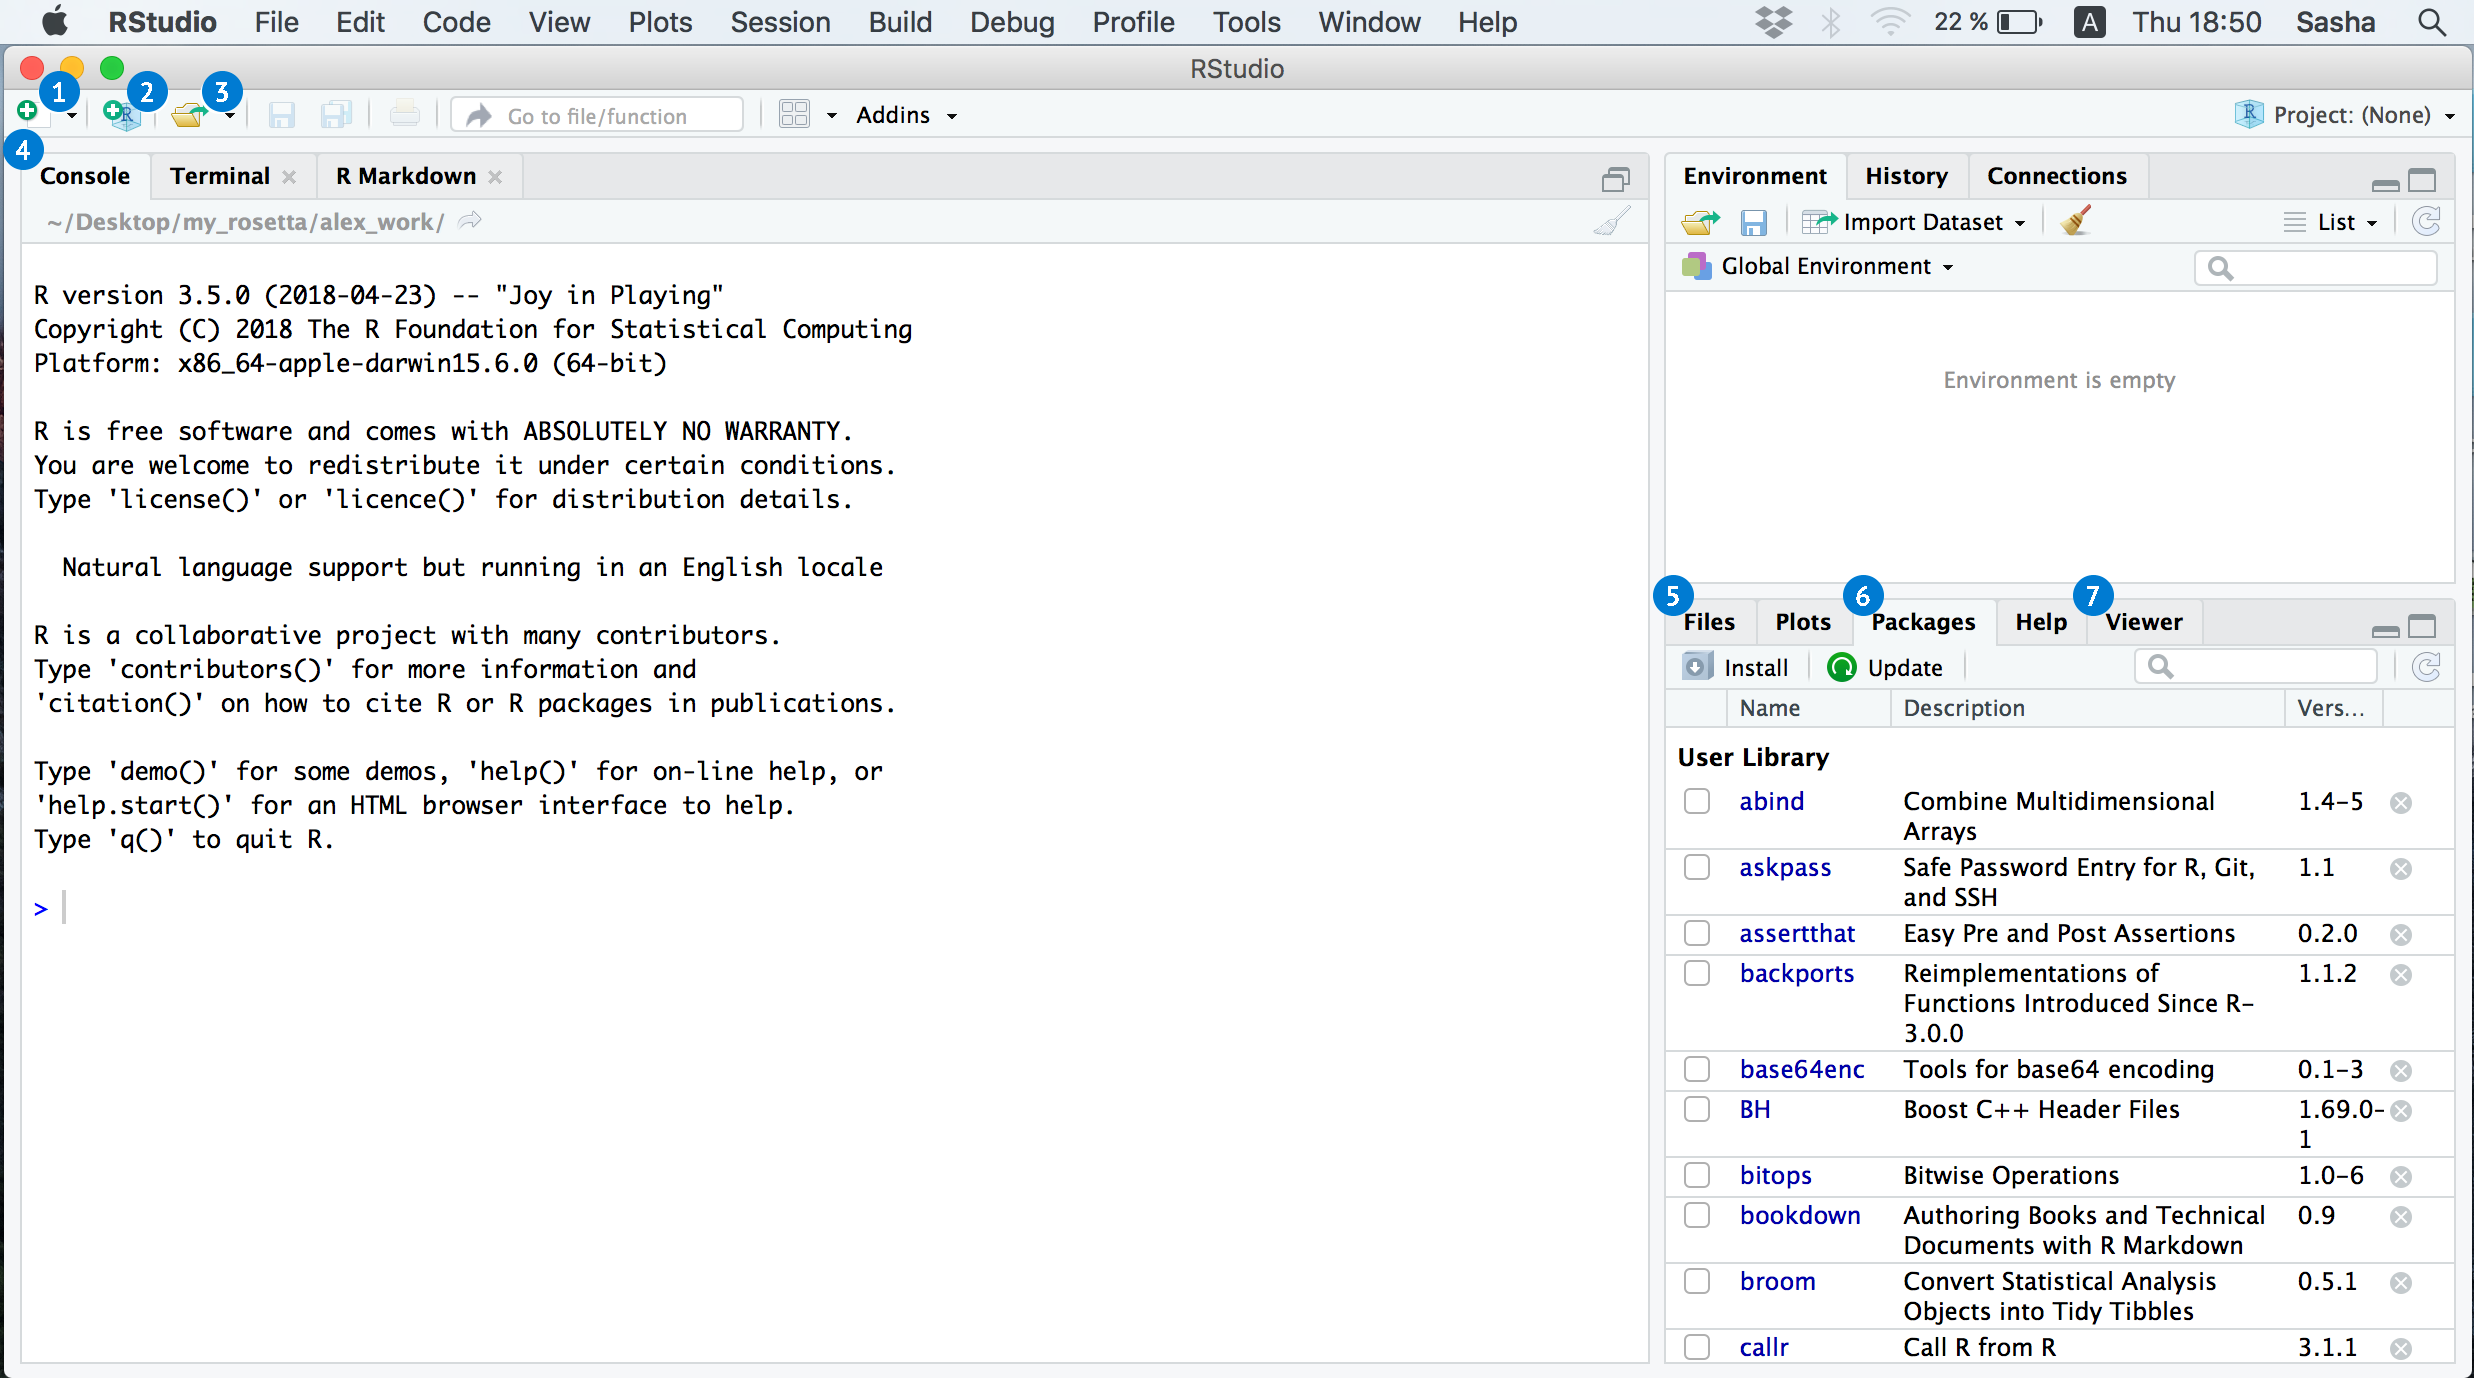
\includegraphics{images/RStudio_Interface.png}
\caption{\emph{Интерфейс программы}}
\end{figure}

\begin{enumerate}
\def\labelenumi{\arabic{enumi}.}
\item
  \textbf{New file} - Создание нового файла.
\item
  \textbf{New project} - Создание нового проекта.
\item
  \textbf{Open file} - Открытие существующего файла.
\item
  \textbf{Console} - Консоль, в которой набирается код.
\item
  \textbf{Files} - Список файлов, доступных для работы.
\item
  \textbf{Packages} - Список установленных пакетов, т.е. расширений. Также можно ознакомиться с ним, введя в консоль команду \emph{installed.packages()}.
\item
  \textbf{Viewer} - Отображение введенного кода.
\end{enumerate}

\begin{center}\rule{0.5\linewidth}{\linethickness}\end{center}

\#\#\#Язык программирования Python
\textgreater{} Python - это ещё одна открытая среда программирования, помогающая в работе со статистическими данными. Для программирования на Python подойдет программа Jupyter Notebook.

\#\#\#\#\#Установка

\begin{enumerate}
\def\labelenumi{\arabic{enumi}.}
\item
  Загрузите и установите Anaconda \href{https://www.anaconda.com/distribution/}{с официального сайта}.
\item
  После загрузки и установки откройте Anaconda Navigator, через который Вы сможете открыть программу Jupyter Notebook.
  
\includegraphics{images/Anaconda Navigator.png}
\end{enumerate}

\#\#\#\#\#Начало работы

Открыв Jupyter Notebook, вы попадете на страницу, содержащую ваши сохраненные файлы. Чтобы создать новый файл, нажмите ``New'' ▶ ``Notebook: Python 3''.
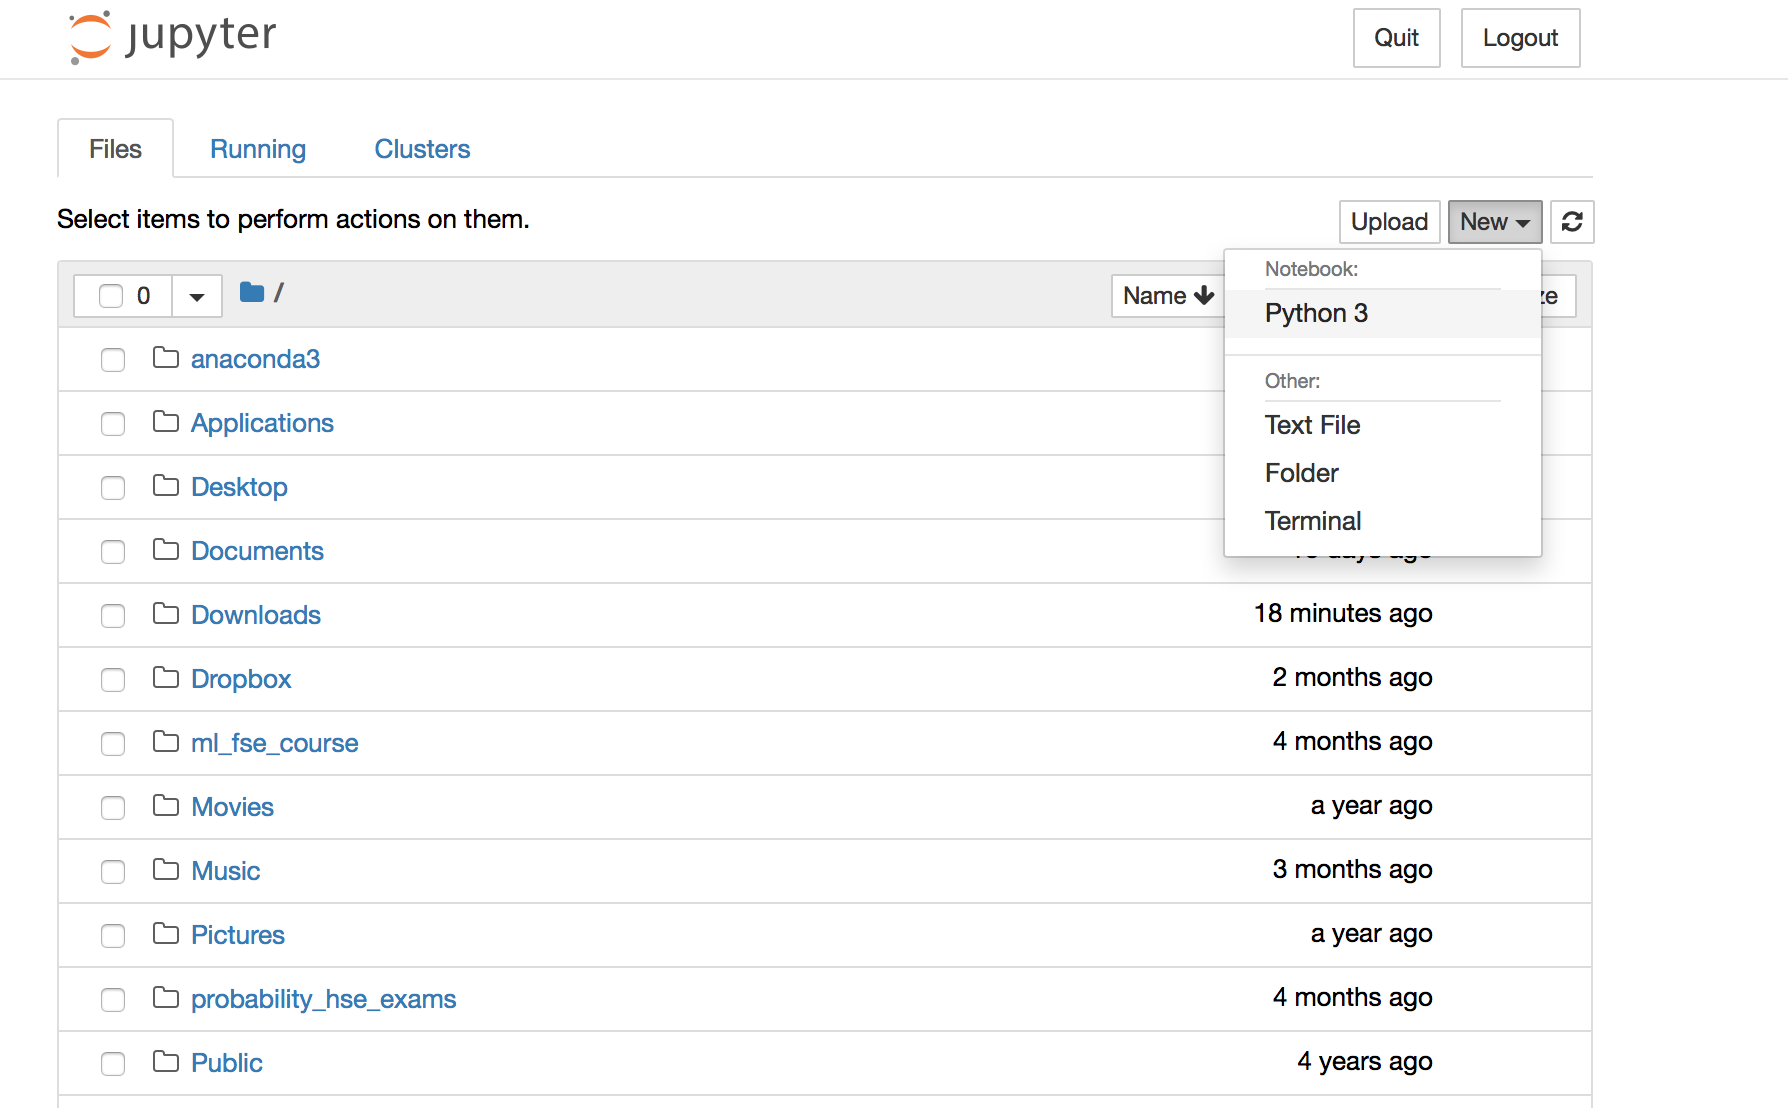
\includegraphics{images/New File in Jupyter.png}

Затем, в открывшемся окне, появится новый файл. Теперь все готово к работе. Вы можете вводить свой код и затем, используя комбинацию клавиш ``Shift'' + ``Enter'', проверять его исполнение.
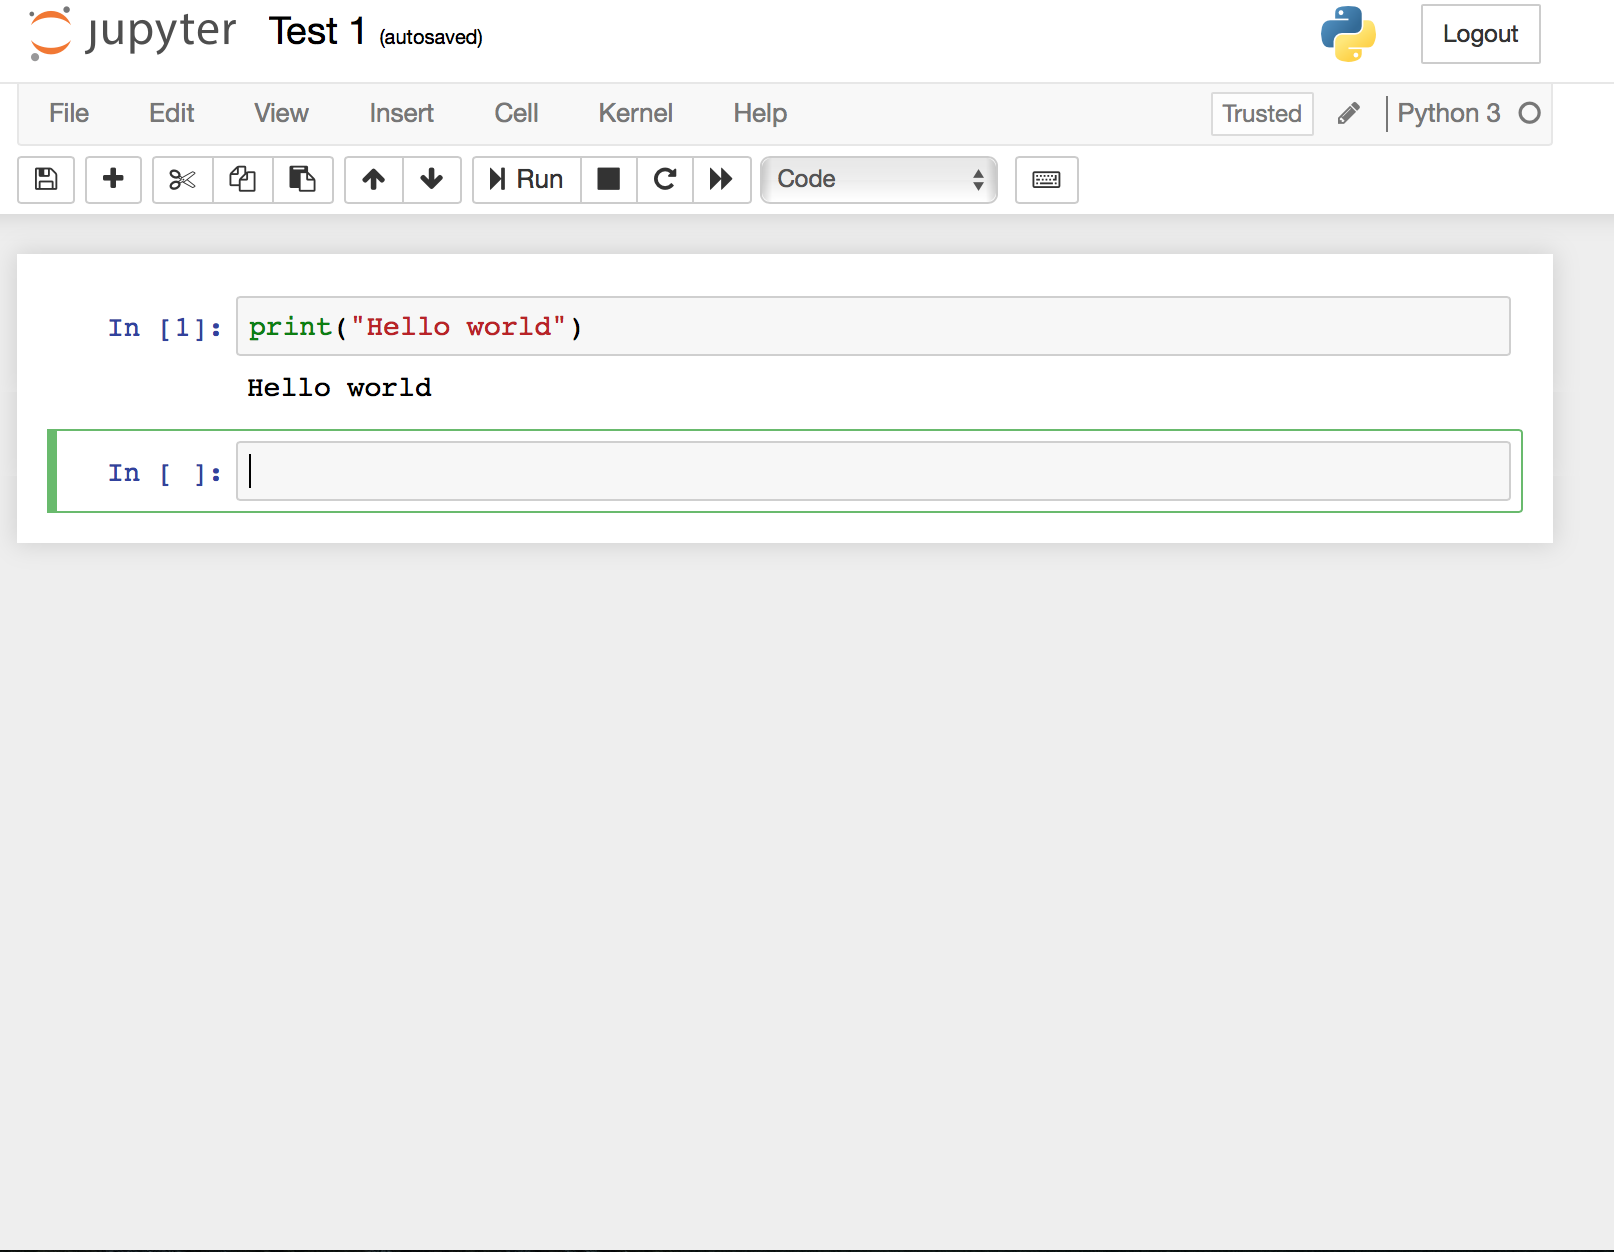
\includegraphics{images/Code in Jupyter.png}

\begin{center}\rule{0.5\linewidth}{\linethickness}\end{center}

\#\#\#Программа STATA
\textgreater{} Stata, в отличие от R и Python, является программой, а не языком программирования. Она также помогает в работе со статистическими данными.

\#\#\#\#\#Установка:

Для установки Stata необходимо загрузить актуальную версию \href{https://www.stata.com/}{с сайта компании-разработчика}. Подойдут как Stata SE, так и Stata MP.

\#\#\#\#\#Начало работы:

\begin{figure}
\centering
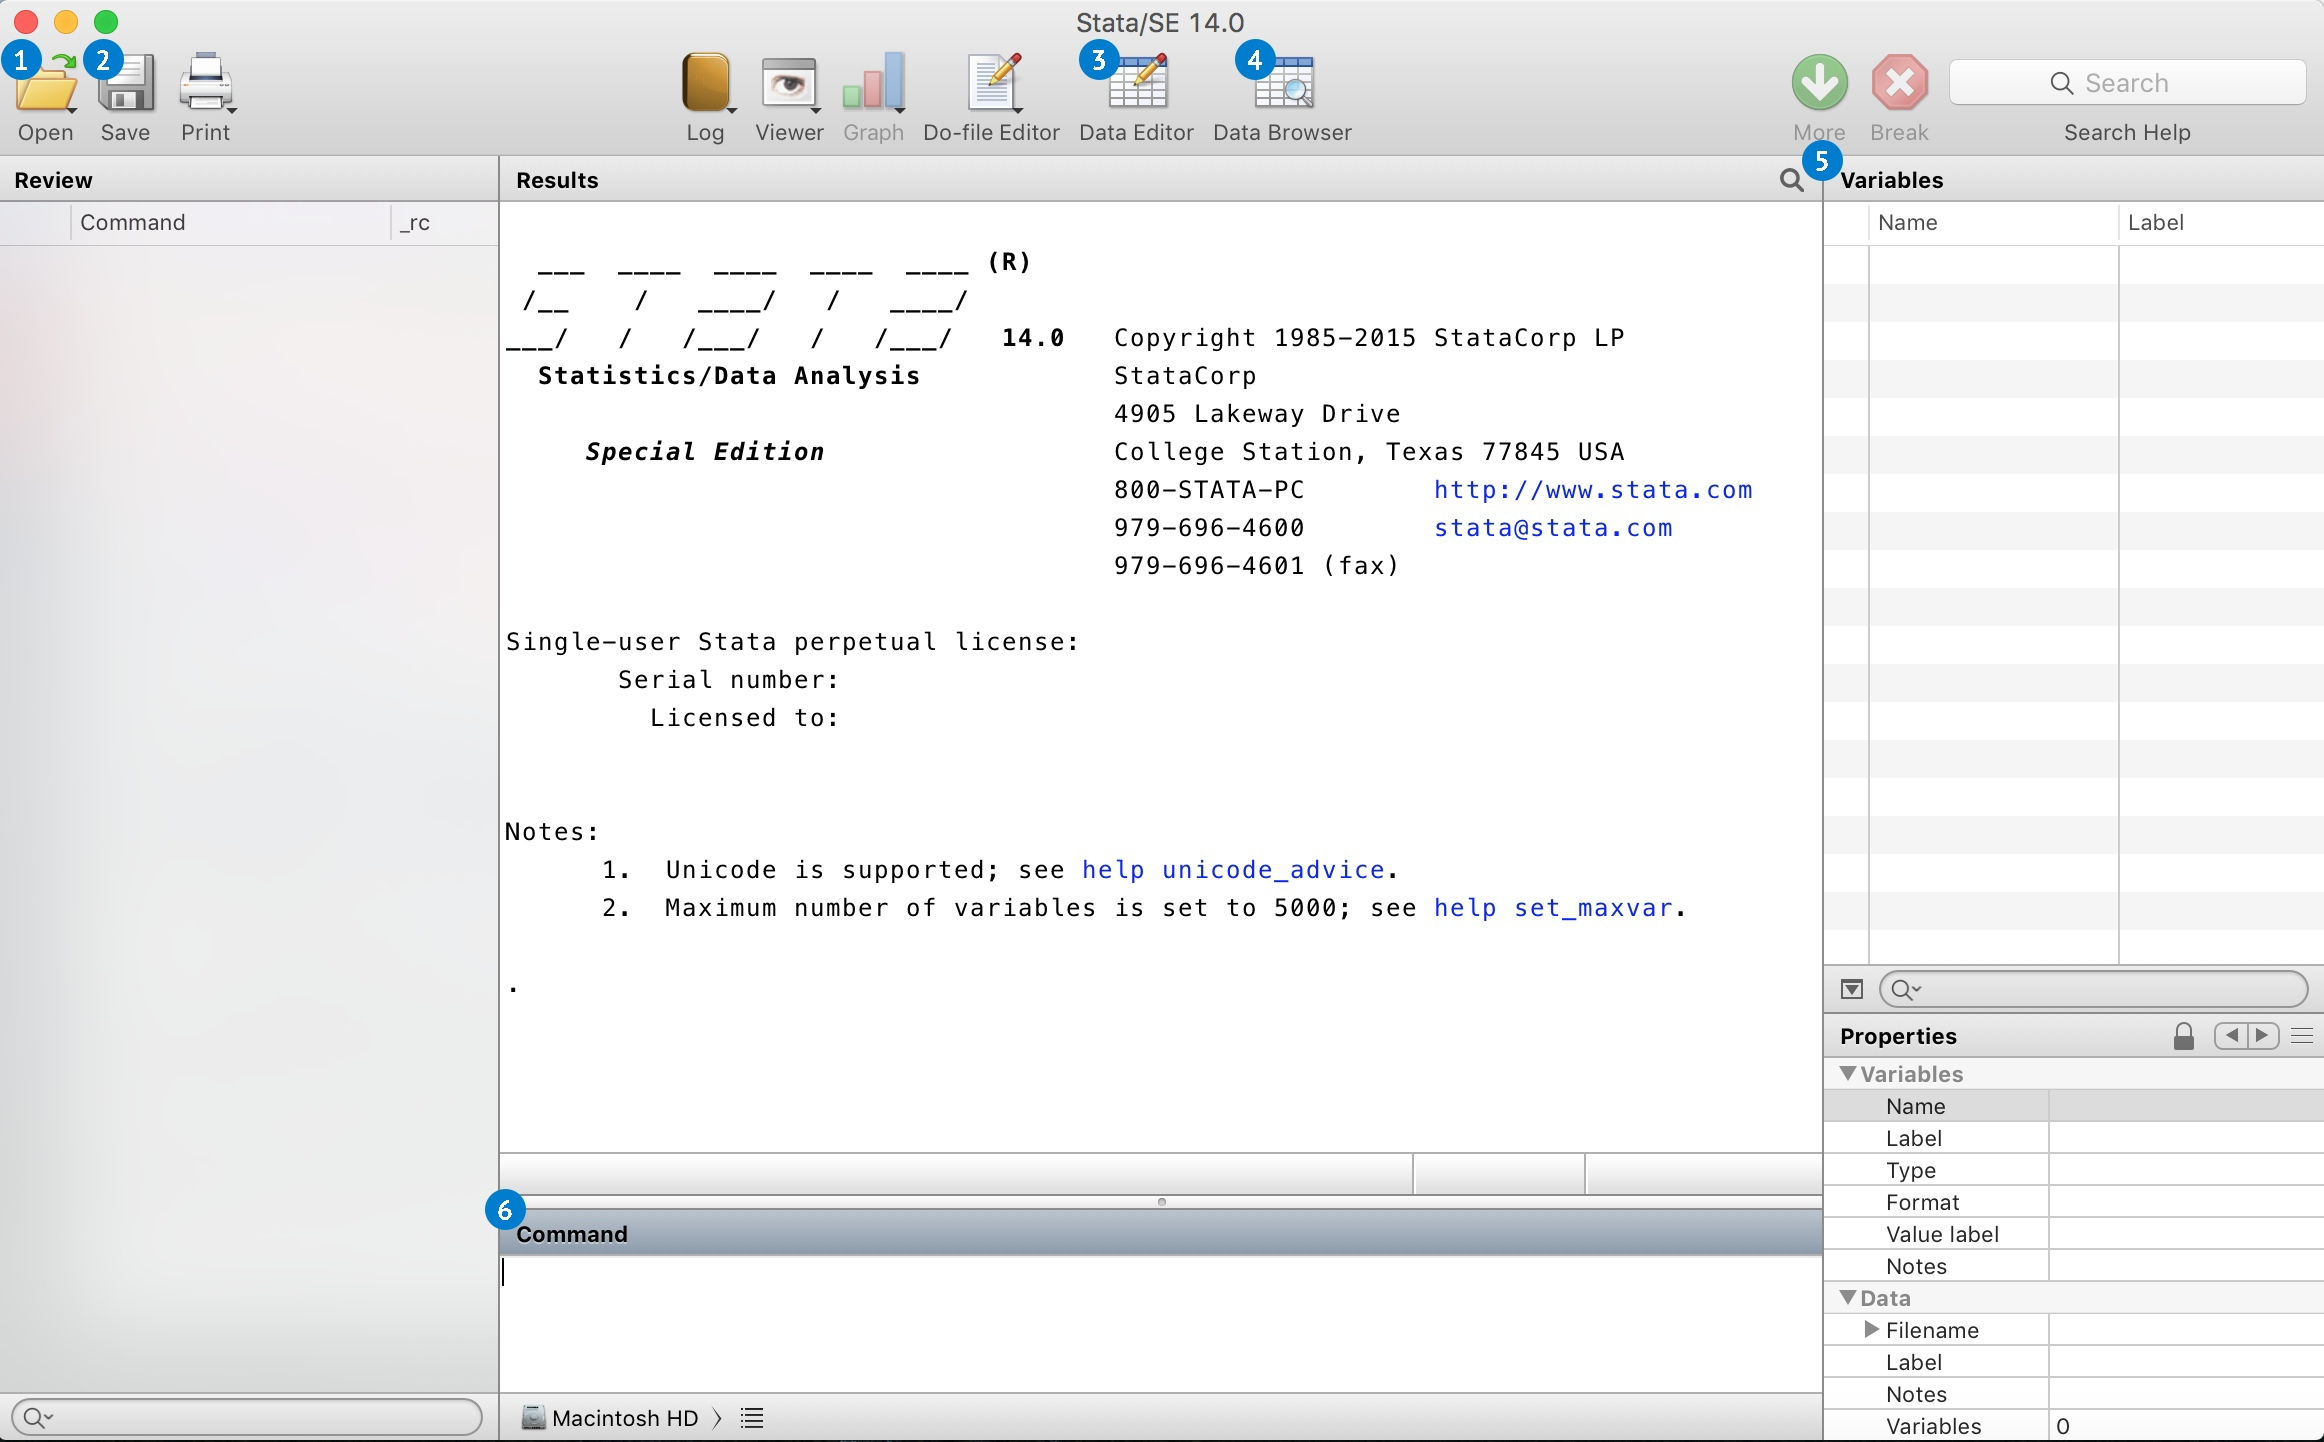
\includegraphics{images/Stata Interface.jpg}
\caption{\emph{Интерфейс Stata}}
\end{figure}

\begin{enumerate}
\def\labelenumi{\arabic{enumi}.}
\tightlist
\item
  \textbf{Open File} - открыть файл.
\item
  \textbf{Save} - сохранить файл.
\item
  \textbf{Data Editor} - редактирование данных.
\item
  \textbf{Data Browser} - просмотр данных.
\item
  \textbf{Variables} - список переменных.
\item
  \textbf{Command} - командная строка, в которой вводится код.
\end{enumerate}

\hypertarget{simplereg}{%
\chapter{Коан о простой линейной регрессии}\label{simplereg}}

Построим простую линейную регрессию в R и проведем несложные тесты.

Загрузим необходимые пакеты.

\begin{Shaded}
\begin{Highlighting}[]
\KeywordTok{library}\NormalTok{(tidyverse) }\CommentTok{# для манипуляций с данными и построения графиков}
\KeywordTok{library}\NormalTok{(skimr) }\CommentTok{# для красивого summary}
\KeywordTok{library}\NormalTok{(rio) }\CommentTok{# для чтения .dta файлов}
\KeywordTok{library}\NormalTok{(car) }\CommentTok{# для линейных гипотез}
\KeywordTok{library}\NormalTok{(tseries) }\CommentTok{# для теста на нормальность}
\KeywordTok{library}\NormalTok{(sjPlot) }\CommentTok{# еще графики}
\end{Highlighting}
\end{Shaded}

Импортируем данные.

\begin{Shaded}
\begin{Highlighting}[]
\NormalTok{df =}\StringTok{ }\KeywordTok{import}\NormalTok{(}\StringTok{"us-return.dta"}\NormalTok{)}
\end{Highlighting}
\end{Shaded}

Исследуем наш датасет.

\begin{Shaded}
\begin{Highlighting}[]
\CommentTok{# skim_with(numeric = list(hist = NULL, p25 = NULL, p75 = NULL)) # опустим некоторые описательные характеристики}
\KeywordTok{skim}\NormalTok{(df) }\CommentTok{# посмотрим на данные}
\end{Highlighting}
\end{Shaded}

\begin{verbatim}
Skim summary statistics
 n obs: 2664 
 n variables: 22 

-- Variable type:character -----------------------------------------------------------------------------------------------------------------------
 variable missing complete    n min max empty n_unique
        B       0     2664 2664   0   6  2544       31

-- Variable type:numeric -------------------------------------------------------------------------------------------------------------------------
 variable missing complete    n    mean      sd      p0     p25     p50
        A    2544      120 2664 60.5    34.79    1      30.75   60.5   
    BOISE    2544      120 2664  0.017   0.097  -0.27   -0.045   0.015 
   CITCRP    2544      120 2664  0.012   0.081  -0.28   -0.037   0.011 
    CONED    2544      120 2664  0.019   0.05   -0.14   -0.012   0.019 
   CONTIL    2544      120 2664 -0.0011  0.15   -0.6    -0.051   0     
   DATGEN    2544      120 2664  0.0075  0.13   -0.34   -0.072   0.017 
      DEC    2544      120 2664  0.02    0.099  -0.36   -0.051   0.024 
    DELTA    2544      120 2664  0.012   0.096  -0.26   -0.053   0.013 
   GENMIL    2544      120 2664  0.017   0.065  -0.15   -0.026   0.011 
   GERBER    2544      120 2664  0.016   0.088  -0.29   -0.036   0.015 
      IBM    2544      120 2664  0.0096  0.059  -0.19   -0.029   0.002 
   MARKET    2544      120 2664  0.014   0.068  -0.26   -0.013   0.012 
    MOBIL    2544      120 2664  0.016   0.08   -0.18   -0.032   0.013 
    MOTOR    2544      120 2664  0.018   0.097  -0.33   -0.053   0.017 
    PANAM    2544      120 2664  0.0035  0.13   -0.31   -0.065   0     
     PSNH    2544      120 2664 -0.0042  0.11   -0.48   -0.049   0     
   rkfree    2544      120 2664  0.0068  0.0022  0.0021  0.0052  0.0066
   RKFREE    2544      120 2664  0.0068  0.0022  0.0021  0.0052  0.0066
    TANDY    2544      120 2664  0.025   0.13   -0.25   -0.058   0.022 
   TEXACO    2544      120 2664  0.012   0.08   -0.19   -0.037   0.01  
    WEYER    2544      120 2664  0.0096  0.085  -0.27   -0.049  -0.002 
     p75    p100     hist
 90.25   120     ▇▇▇▇▇▇▇▇
  0.07     0.38  ▁▂▆▇▇▂▁▁
  0.064    0.32  ▁▁▅▇▇▃▁▁
  0.045    0.15  ▁▁▂▇▇▅▂▂
  0.058    0.97  ▁▁▇▇▁▁▁▁
  0.078    0.53  ▁▂▅▇▃▁▁▁
  0.075    0.39  ▁▁▂▇▇▂▁▁
  0.063    0.29  ▁▂▅▇▇▃▂▁
  0.06     0.19  ▁▃▅▇▅▃▂▁
  0.065    0.23  ▁▁▁▅▇▅▂▁
  0.05     0.15  ▁▁▂▇▇▆▃▂
  0.062    0.15  ▁▁▁▂▅▇▇▂
  0.057    0.37  ▁▃▇▇▂▁▁▁
  0.084    0.27  ▁▁▂▇▇▇▃▁
  0.074    0.41  ▁▂▅▇▃▁▁▁
  0.043    0.32  ▁▁▁▁▇▆▁▁
  0.0078   0.013 ▁▃▆▇▅▂▂▂
  0.0078   0.013 ▁▃▆▇▅▂▂▂
  0.094    0.45  ▂▃▆▇▂▂▁▁
  0.048    0.4   ▁▃▇▆▂▁▁▁
  0.06     0.27  ▁▁▅▇▆▃▂▁
\end{verbatim}

\begin{Shaded}
\begin{Highlighting}[]
\NormalTok{df =}\StringTok{ }\KeywordTok{rename}\NormalTok{(df, }\DataTypeTok{n =}\NormalTok{ A, }\DataTypeTok{date =}\NormalTok{ B) }\CommentTok{# дадим столбцам более осмысленные названия}
\end{Highlighting}
\end{Shaded}

\begin{Shaded}
\begin{Highlighting}[]
\NormalTok{df =}\StringTok{ }\KeywordTok{na.omit}\NormalTok{(df) }\CommentTok{# уберем строки с пропущенными наблюдениями}
\end{Highlighting}
\end{Shaded}

Будем верить в CAPM :) Оценим параметры модели для компании MOTOR. Соответственно, зависимая переменная - разница доходностей акций MOTOR и безрискового актива, а регрессор - рыночная премия.

\begin{Shaded}
\begin{Highlighting}[]
\CommentTok{#создаем новые переменные и добавляем их к набору данных}
\NormalTok{df =}\StringTok{ }\KeywordTok{mutate}\NormalTok{(df, }\DataTypeTok{y =}\NormalTok{ MOTOR }\OperatorTok{-}\StringTok{ }\NormalTok{RKFREE, }\DataTypeTok{x =}\NormalTok{ MARKET }\OperatorTok{-}\StringTok{ }\NormalTok{RKFREE) }
\end{Highlighting}
\end{Shaded}

Строим нашу модель и проверяем гипотезу об адекватности регрессии.

\begin{Shaded}
\begin{Highlighting}[]
\NormalTok{ols =}\StringTok{ }\KeywordTok{lm}\NormalTok{(y }\OperatorTok{~}\StringTok{ }\NormalTok{x, }\DataTypeTok{data =}\NormalTok{ df)}
\KeywordTok{summary}\NormalTok{(ols)}
\end{Highlighting}
\end{Shaded}

\begin{verbatim}

Call:
lm(formula = y ~ x, data = df)

Residuals:
      Min        1Q    Median        3Q       Max 
-0.168421 -0.059381 -0.003399  0.061373  0.182991 

Coefficients:
            Estimate Std. Error t value Pr(>|t|)    
(Intercept) 0.005253   0.007200   0.730    0.467    
x           0.848150   0.104814   8.092 5.91e-13 ***
---
Signif. codes:  0 '***' 0.001 '**' 0.01 '*' 0.05 '.' 0.1 ' ' 1

Residual standard error: 0.07844 on 118 degrees of freedom
Multiple R-squared:  0.3569,    Adjusted R-squared:  0.3514 
F-statistic: 65.48 on 1 and 118 DF,  p-value: 5.913e-13
\end{verbatim}

Вызовом одной функции получаем кучу полезных графиков. Можем визуально оценить наличие гетероскедастичности, нормальность распределения остатков, наличие выбросов.

\begin{Shaded}
\begin{Highlighting}[]
\KeywordTok{plot}\NormalTok{(ols)}
\end{Highlighting}
\end{Shaded}

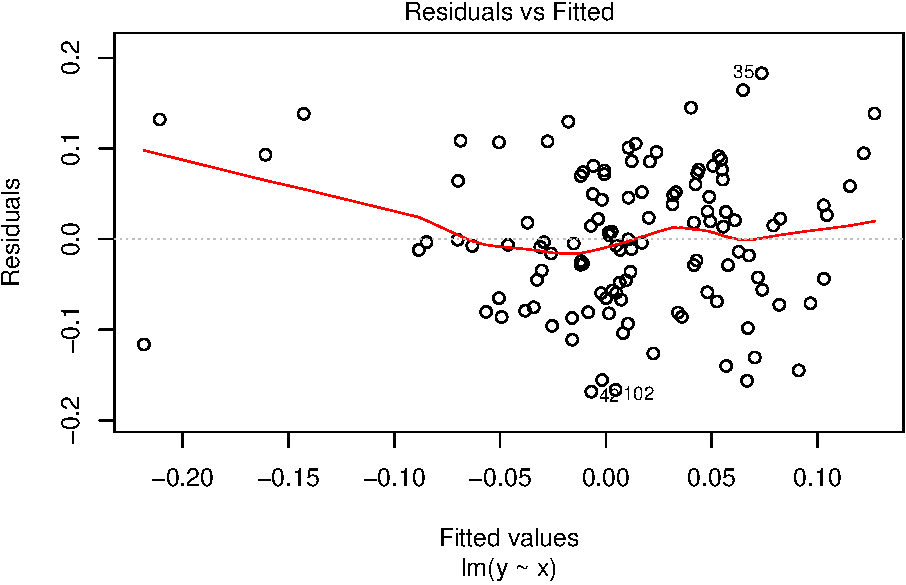
\includegraphics{02-simplereg_files/figure-latex/plot-1.pdf} 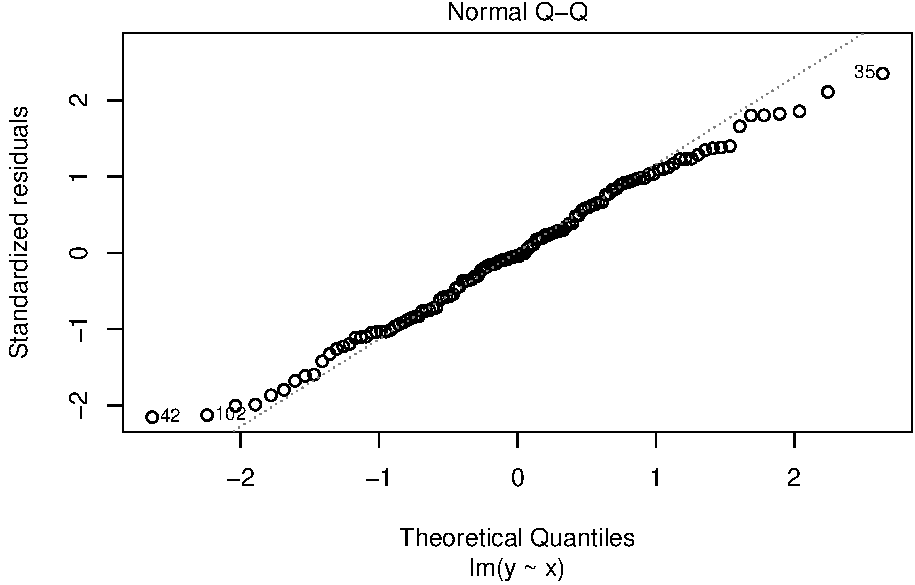
\includegraphics{02-simplereg_files/figure-latex/plot-2.pdf} 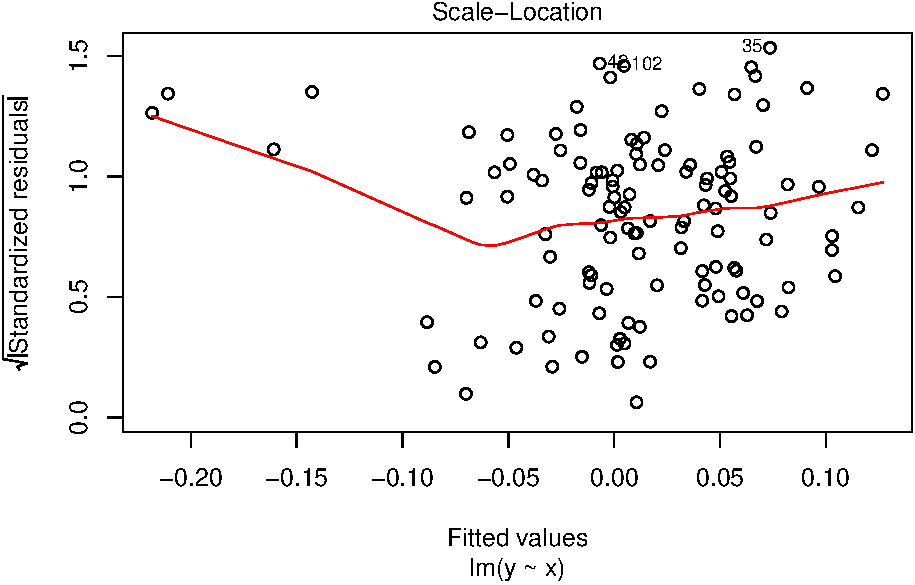
\includegraphics{02-simplereg_files/figure-latex/plot-3.pdf} 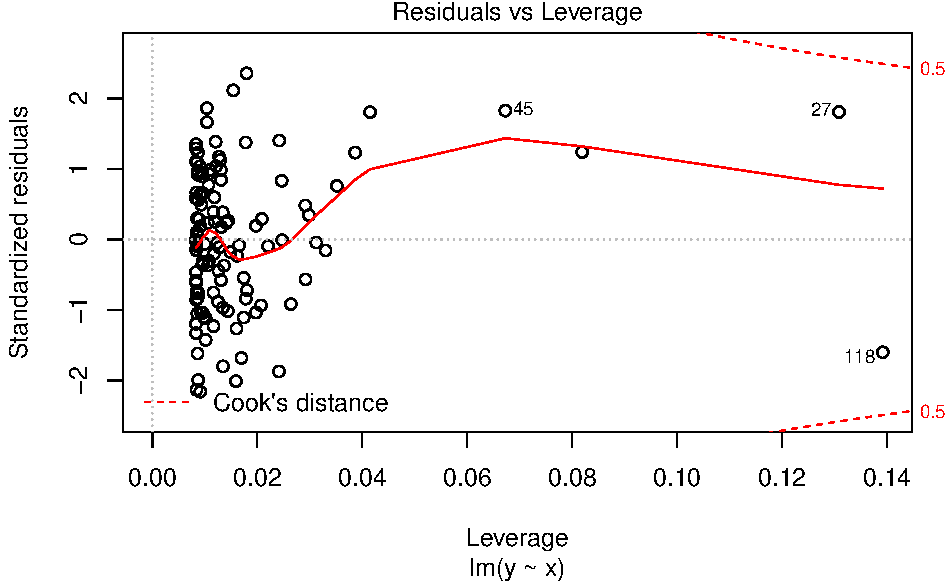
\includegraphics{02-simplereg_files/figure-latex/plot-4.pdf}

Строим доверительный интервал для параметров модели.

\begin{Shaded}
\begin{Highlighting}[]
\NormalTok{est =}\StringTok{ }\KeywordTok{cbind}\NormalTok{(}\DataTypeTok{Estimate =} \KeywordTok{coef}\NormalTok{(ols), }\KeywordTok{confint}\NormalTok{(ols))}
\end{Highlighting}
\end{Shaded}

Проверим гипотезу о равенстве коэффициента при регрессоре единице.

\begin{Shaded}
\begin{Highlighting}[]
\KeywordTok{linearHypothesis}\NormalTok{(ols, }\KeywordTok{c}\NormalTok{(}\StringTok{"x = 1"}\NormalTok{))}
\end{Highlighting}
\end{Shaded}

\begin{verbatim}
Linear hypothesis test

Hypothesis:
x = 1

Model 1: restricted model
Model 2: y ~ x

  Res.Df     RSS Df Sum of Sq      F Pr(>F)
1    119 0.73900                           
2    118 0.72608  1  0.012915 2.0989 0.1501
\end{verbatim}

Посмотрим на остатки :) Протестируем остатки регрессии на нормальность с помощью теста Харке-Бера.

\[
H_{0}: S = 0, K = 3,
\]
где \(S\) --- коэффициент асимметрии (Skewness), \(K\) --- коэффициент эксцесса (Kurtosis)

\begin{Shaded}
\begin{Highlighting}[]
\KeywordTok{jarque.bera.test}\NormalTok{(}\KeywordTok{resid}\NormalTok{(ols)) }
\end{Highlighting}
\end{Shaded}

\begin{verbatim}

    Jarque Bera Test

data:  resid(ols)
X-squared = 1.7803, df = 2, p-value = 0.4106
\end{verbatim}

И тест Шапиро-Уилка.

\(H_{0}: \epsilon_{i} \sim N(\mu,\sigma^2)\)

\begin{Shaded}
\begin{Highlighting}[]
\KeywordTok{shapiro.test}\NormalTok{(}\KeywordTok{resid}\NormalTok{(ols))}
\end{Highlighting}
\end{Shaded}

\begin{verbatim}

    Shapiro-Wilk normality test

data:  resid(ols)
W = 0.99021, p-value = 0.5531
\end{verbatim}

Оба теста указывают на нормальность распределения остатков регрессии.

Сделаем прогноз модели по данным вне обучаемой выборки.

\begin{Shaded}
\begin{Highlighting}[]
\KeywordTok{set.seed}\NormalTok{(}\DecValTok{7}\NormalTok{)}
\NormalTok{newData =}\StringTok{ }\NormalTok{df}
\NormalTok{newData =}\StringTok{ }\KeywordTok{mutate}\NormalTok{(newData, }\DataTypeTok{x =}\NormalTok{ x }\OperatorTok{+}\StringTok{ }\KeywordTok{rnorm}\NormalTok{(}\DataTypeTok{n =} \KeywordTok{n}\NormalTok{())) }\CommentTok{# пошумим}
\NormalTok{yhat =}\StringTok{ }\KeywordTok{predict}\NormalTok{(ols, }\DataTypeTok{newdata =}\NormalTok{ newData, }\DataTypeTok{se =} \OtherTok{TRUE}\NormalTok{)}
\end{Highlighting}
\end{Shaded}

\hypertarget{----}{%
\subsubsection{То же самое в стате}\label{----}}

Загружаем данные.

\begin{verbatim}
use us-return.dta
\end{verbatim}

\begin{verbatim}
end of do-file
\end{verbatim}

Любуемся и даем новые названия столбцам.

\begin{verbatim}
summarize
ren A n
ren B date
\end{verbatim}

\begin{verbatim}
    Variable |        Obs        Mean    Std. Dev.       Min        Max
-------------+---------------------------------------------------------
           A |        120        60.5    34.78505          1        120
           B |          0
       MOBIL |        120    .0161917    .0803075      -.178       .366
      TEXACO |        120    .0119417    .0797036      -.194       .399
         IBM |        120    .0096167     .059024      -.187        .15
-------------+---------------------------------------------------------
         DEC |        120      .01975    .0991438      -.364       .385
      DATGEN |        120    .0074833    .1275399      -.342       .528
       CONED |        120    .0185083    .0502719      -.139       .151
        PSNH |        120   -.0042167    .1094712      -.485       .318
       WEYER |        120    .0096333    .0850664      -.271        .27
-------------+---------------------------------------------------------
       BOISE |        120     .016675    .0974882      -.274       .379
       MOTOR |        120    .0181583    .0972656      -.331        .27
       TANDY |        120    .0250083     .127566      -.246       .454
       PANAM |        120    .0035167    .1318054      -.313       .406
       DELTA |        120    .0116917    .0959317       -.26       .289
-------------+---------------------------------------------------------
      CONTIL |        120      -.0011    .1506992        -.6       .974
      CITCRP |        120    .0118583    .0809719      -.282       .318
      GERBER |        120       .0164    .0877379      -.288       .234
      GENMIL |        120    .0165833    .0650403      -.148        .19
      MARKET |        120    .0139917    .0683532       -.26       .148
-------------+---------------------------------------------------------
      RKFREE |        120    .0068386    .0021869     .00207     .01255
      rkfree |        120    .0068386    .0021869     .00207     .01255
\end{verbatim}

Убираем пропущенные значения и создаем новые переменные.

\begin{verbatim}
drop if n == .
gen y = MOTOR - RKFREE
gen x = MARKET - RKFREE
\end{verbatim}

\begin{verbatim}
(2,544 observations deleted)
\end{verbatim}

Строим модель и проверяем гипотезу об адекватности регрессии. Тут же получаем доверительные интервалы для коэффициентов.

\begin{verbatim}
reg y x
\end{verbatim}

\begin{verbatim}
      Source |       SS           df       MS      Number of obs   =       120
-------------+----------------------------------   F(1, 118)       =     65.48
       Model |  .402913404         1  .402913404   Prob > F        =    0.0000
    Residual |  .726081541       118  .006153233   R-squared       =    0.3569
-------------+----------------------------------   Adj R-squared   =    0.3514
       Total |  1.12899494       119  .009487352   Root MSE        =    .07844

------------------------------------------------------------------------------
           y |      Coef.   Std. Err.      t    P>|t|     [95% Conf. Interval]
-------------+----------------------------------------------------------------
           x |   .8481496   .1048138     8.09   0.000     .6405898    1.055709
       _cons |   .0052529   .0071999     0.73   0.467     -.009005    .0195107
------------------------------------------------------------------------------
\end{verbatim}

Проверим гипотезу о равенстве коэффициента при регрессоре единице.

\begin{verbatim}
test x = 1
\end{verbatim}

\begin{verbatim}
 ( 1)  x = 1

       F(  1,   118) =    2.10
            Prob > F =    0.1501
\end{verbatim}

Сделаем предсказание по выборке и сохраним остатки.

\begin{verbatim}
predict u_hat, resid
predict y_hat
\end{verbatim}

\begin{verbatim}
(option xb assumed; fitted values)
\end{verbatim}

Протестируем остатки регрессии на нормальность с помощью теста Харке-Бера.
На самом деле, это не совсем тест Харке-Бера. Оригинальный вариант ассимптотический и в нем нет поправки на размер выборки. В Stata есть. Подробнее здесь \url{https://www.stata.com/manuals13/rsktest.pdf}

\begin{verbatim}
sktest u_hat
\end{verbatim}

\begin{verbatim}
                    Skewness/Kurtosis tests for Normality
                                                          ------ joint ------
    Variable |        Obs  Pr(Skewness)  Pr(Kurtosis) adj chi2(2)   Prob>chi2
-------------+---------------------------------------------------------------
       u_hat |        120     0.8841        0.1027        2.74         0.2539
\end{verbatim}

И тест Шапиро-Уилка. Тут все аналогично R.

\begin{verbatim}
swilk u_hat
\end{verbatim}

\begin{verbatim}
                   Shapiro-Wilk W test for normal data

    Variable |        Obs       W           V         z       Prob>z
-------------+------------------------------------------------------
       u_hat |        120    0.99021      0.942    -0.133    0.55310
\end{verbatim}

Гипотеза о нормальности остатков не отвергается.

QQ - график

\begin{verbatim}
qnorm u_hat 
\end{verbatim}

\begin{verbatim}

График предсказанных значений против остатков.

```stata
rvfplot, yline(0)
```
\end{verbatim}

График диагональных элементов матрицы-шляпницы против квадрата остатков (по сравнению с R оси поменялись местами).

\begin{verbatim}
lvr2plot
\end{verbatim}

\begin{verbatim}

График предсказанных значений против стандартизиованных остатков. Размер точек на графике зависит от расстояния Кука для данного наблюдения.

```stata
predict D, cooksd
predict standard, rstandard

graph twoway scatter standard y_hat [aweight=D], msymbol(oh) yline(0)
```

```

```



```stata
set seed 7

set obs 120
gen x_new = x+ 0.5 *rnormal()
gen y_hat_new =  .8481496 * x_new+ .0052529
```

```
number of observations (_N) was 120, now 120

```
#### То же самое в python

Много хорошихх функций для статистических расчетов можно найти в пакете Statsmodels. 

```python

import pandas as pd # для работы с таблицами
import numpy as np # математика, работа с матрицами
import matplotlib.pyplot as plt # графики
import statsmodels.api as sm
import statsmodels.formula.api as smf
import statsmodels.graphics.gofplots as gf
from statsmodels.stats.outliers_influence import summary_table
import seaborn as sns # еще более классные графики
from scipy.stats import shapiro # еще математика
import statsmodels.discrete.discrete_model
```

При желании, можем кастомизировать графики :)

```python
plt.style.use('seaborn')
plt.rc('font', size=14)
plt.rc('figure', titlesize=15)
plt.rc('axes', labelsize=15)
plt.rc('axes', titlesize=15)
```

Загрузим данные.

```python
df = pd.read_stata('us-return.dta')
```

Избавимся от наблюдений с пропущенными значенями. 

```python
df.dropna(inplace=True) ##ИСПРАВИТЬ (выкинуть только пропуски целевой и объяснющей)
df.reset_index(drop=True, inplace=True)
```

Переименуем столбцы.

```python
df = df.rename(columns={'A':'n', 'B': 'date'})
```


```python
df['y'] = df['MOTOR'] - df['RKFREE']
df['x'] = df['MARKET'] - df['RKFREE'] 
```

Строим модель и читаем саммари :)

```python
regr = smf.ols('y~x', data = df).fit()
regr.summary()
```

```
<class 'statsmodels.iolib.summary.Summary'>
"""
                            OLS Regression Results                            
==============================================================================
Dep. Variable:                      y   R-squared:                       0.357
Model:                            OLS   Adj. R-squared:                  0.351
Method:                 Least Squares   F-statistic:                     65.48
Date:                 Пн, 16 сен 2019   Prob (F-statistic):           5.91e-13
Time:                        15:59:27   Log-Likelihood:                 136.18
No. Observations:                 120   AIC:                            -268.4
Df Residuals:                     118   BIC:                            -262.8
Df Model:                           1                                         
Covariance Type:            nonrobust                                         
==============================================================================
                 coef    std err          t      P>|t|      [0.025      0.975]
------------------------------------------------------------------------------
Intercept      0.0053      0.007      0.730      0.467      -0.009       0.020
x              0.8481      0.105      8.092      0.000       0.641       1.056
==============================================================================
Omnibus:                        2.684   Durbin-Watson:                   2.030
Prob(Omnibus):                  0.261   Jarque-Bera (JB):                1.780
Skew:                          -0.031   Prob(JB):                        0.411
Kurtosis:                       2.406   Cond. No.                         14.6
==============================================================================

Warnings:
[1] Standard Errors assume that the covariance matrix of the errors is correctly specified.
"""
```

Получить прогноз.

```python
df['yhat'] = regr.fittedvalues
```

Красивые графики для остатков, выборосов и прочих радостей, как в R, придется строить ручками. Зато приятно поиграть с оформлением :)

```python
fig, ax = plt.subplots()
ax.plot(df['x'],regr.fittedvalues, color='g', alpha =0.8)
ax.scatter(df['x'],regr.fittedvalues+regr.resid, color = 'g', alpha = 0.8, s = 40)
ax.vlines(df['x'],regr.fittedvalues,regr.fittedvalues+regr.resid, color = 'gray', alpha = 0.5)
plt.title('Линия регрессии и остатки')
plt.xlabel('RKFREE')
plt.ylabel('MARKET')
plt.show()
```

![](02-simplereg_files/figure-latex/unnamed-chunk-13-1.pdf)<!-- --> 

Строим доверительный интервал.

```python
regr.conf_int()
```

```
                  0         1
Intercept -0.009005  0.019511
x          0.640590  1.055709
```

И проведем F-test.

```python
hypotheses = '(x = 1)'
regr.f_test(r_matrix = hypotheses)
```

```
<class 'statsmodels.stats.contrast.ContrastResults'>
<F test: F=array([[2.09891771]]), p=0.1500556415866233, df_denom=118, df_num=1>
```

Тест Шапиро. Такой же, как и в R. Для удобства можно поместить в табличку.

```python
W, p_value = shapiro(regr.resid)
#pd.DataFrame(data = {'W': [round(W,3)], 'p_value': [round(p_value,3)]})
```


Генерируем новые данные и строим предсказание.

```python
import random
random.seed(7)

newData = df['x'] + 0.5*np.random.normal(len(df))
prediction = regr.predict(newData)
```

А теперь жесть! Построим графички, похожие на autoplot R.


```python
fig_1 = plt.figure(1)

fig_1.axes[0] = sns.residplot(df['x'], df['y'],
                                  lowess=True,
                                  scatter_kws={'alpha': 0.6},
                                  line_kws={'color': 'red', 'lw': 2, 'alpha': 0.8})

fig_1.axes[0].set_title('Residuals vs Fitted')
fig_1.axes[0].set_xlabel('Fitted values')
fig_1.axes[0].set_ylabel('Residuals')


#можем добавить метки потенциальных аутлаеров
abs_resid = abs(regr.resid).sort_values(ascending=False)
abs_resid_top3 = abs_resid[:3]

for i in abs_resid_top3.index:
    fig_1.axes[0].annotate(i, 
                               xy=(regr.fittedvalues[i], 
                                   regr.resid[i]))
```

![](02-simplereg_files/figure-latex/unnamed-chunk-18-1.pdf)<!-- --> 



```python
norm_residuals = regr.get_influence().resid_studentized_internal #сохраним стьюдентизированные остатки 


QQ = gf.ProbPlot(norm_residuals)
fig_2 = QQ.qqplot(line='45', alpha=0.5, color='b', lw=1)


fig_2.axes[0].set_title('Normal Q-Q')
fig_2.axes[0].set_xlabel('Theoretical Quantiles')
fig_2.axes[0].set_ylabel('Standardized Residuals');

#и снова метки
abs_norm_resid = np.flip(np.argsort(abs(norm_residuals)), 0)
abs_norm_resid_top3 = abs_norm_resid[:3]

for r, i in enumerate(abs_norm_resid_top3):
    fig_2.axes[0].annotate(i, 
                               xy=(np.flip(QQ.theoretical_quantiles, 0)[r],
                                   norm_residuals[i]))
```

![](02-simplereg_files/figure-latex/unnamed-chunk-19-1.pdf)<!-- --> 



```python
fig_3 = plt.figure(3)

plt.scatter(regr.fittedvalues, np.sqrt(abs(norm_residuals)), alpha=0.5)
sns.regplot(regr.fittedvalues, np.sqrt(abs(norm_residuals)), 
            scatter=False, 
            ci=False, 
            lowess=True,
            line_kws={'color': 'red', 'lw': 1, 'alpha': 0.6})

fig_3.axes[0].set_title('Scale-Location')
fig_3.axes[0].set_xlabel('Fitted values')
fig_3.axes[0].set_ylabel('$\sqrt{|Standardized Residuals|}$')

# и еще раз!)
abs_sq_norm_resid = np.flip(np.argsort(np.sqrt(abs(norm_residuals)), 0))
abs_sq_norm_resid_top3 = abs_sq_norm_resid[:3]

for i in abs_sq_norm_resid_top3:
    fig_3.axes[0].annotate(i, xy=(regr.fittedvalues[i], 
                                   np.sqrt(abs(norm_residuals)[i])))
```

![](02-simplereg_files/figure-latex/unnamed-chunk-20-1.pdf)<!-- --> 


```python
leverage = regr.get_influence().hat_matrix_diag #сохраняем элементы матрицы-шляпницы
cook_dist = regr.get_influence().cooks_distance[0] #И расстояние Кука

fig_4 = plt.figure(4)

plt.scatter(leverage, norm_residuals, alpha=0.5)
sns.regplot(leverage, norm_residuals, 
            scatter=False, 
            ci=False, 
            lowess=True,
            line_kws={'color': 'red', 'lw': 1, 'alpha': 0.8})

fig_4.axes[0].set_xlim(0, 0.20)
```

```
(0, 0.2)
```

```python
fig_4.axes[0].set_ylim(-3, 5)
```

```
(-3, 5)
```

```python
fig_4.axes[0].set_title('Residuals vs Leverage')
fig_4.axes[0].set_xlabel('Leverage')
fig_4.axes[0].set_ylabel('Standardized Residuals')


leverage_top3 = np.flip(np.argsort(cook_dist), 0)[:3]

for i in leverage_top3:
    fig_4.axes[0].annotate(i, 
                               xy=(leverage[i], 
                                   norm_residuals[i]))
plt.show()
```

![](02-simplereg_files/figure-latex/unnamed-chunk-21-1.pdf)<!-- --> 


<!--chapter:end:02-simplereg.Rmd-->

# Модели бинарного выбора {#binchoice}


<!--chapter:end:03-binchoice.Rmd-->

# Модели упорядоченного выбора и условный логит {#ordchoice}




Загрузим необходимые пакеты.

```r
library(tidyverse) # для манипуляций с данными и построения графиков
library(skimr) #для красивого summary
library(rio) # для чтения .dta файлов
library(margins)
```

```
Error in library(margins): there is no package called 'margins'
```

```r
library(mlogit)
```

```
Error in library(mlogit): there is no package called 'mlogit'
```

```r
library(nnet)
library(questionr)
```

```
Error in library(questionr): there is no package called 'questionr'
```

```r
library(MASS)
library(survival)

# log(6)
```

Импортируем датасет. В нем находятся данные по клиентам пенсионных фондов. Нас интересует переменная `pctstck`, которая принимает три значения: 0, 50, 100 - в зависимоcти от ответа респондента на вопрос о предпочтительном способе инвестирования пенсионных накоплений.   

```r
df = rio::import("pension.dta")
```


```r
skim_with(numeric = list(hist = NULL, p25 = NULL, p75 = NULL)) #посмотрим на данные
#skim(df)
```


Создадим факторную перменную и упорядочим категории. 


```r
df = rename(df,  alloc = pctstck) # переименуем 
df = mutate(df, alloc_factor = factor(alloc)) # факторная переменная
df = mutate(df, y = relevel(df$alloc_factor, ref = 1)) # сменить базовую категорию
levels(df$y)
```

```
[1] "0"   "50"  "100"
```

Построим модель множественного выбора (лог-линейная модель). 

```r
multmodel = multinom(y ~ choice+age+educ+wealth89+prftshr, data = df)
```

```
# weights:  21 (12 variable)
initial  value 220.821070 
iter  10 value 207.012642
iter  20 value 204.507792
final  value 204.507779 
converged
```

```r
summary(multmodel)
```

```
Call:
multinom(formula = y ~ choice + age + educ + wealth89 + prftshr, 
    data = df)

Coefficients:
    (Intercept)    choice         age       educ      wealth89    prftshr
50     3.777686 0.6269410 -0.10621691 0.18518113 -0.0003716626 -0.2717872
100    4.492971 0.6244954 -0.09482129 0.04644315 -0.0003548369  0.9809245

Std. Errors:
    (Intercept)    choice        age       educ     wealth89   prftshr
50     1.581691 0.3701263 0.02826469 0.06725443 0.0007365833 0.4988234
100    1.385291 0.3851273 0.02530600 0.07203058 0.0007896235 0.4396202

Residual Deviance: 409.0156 
AIC: 433.0156 
```

Сохраним прогнозы.

```r
fit_values = fitted(multmodel)
head(fit_values)
```

```
          0        50       100
1 0.4040703 0.3308134 0.2651163
2 0.1534943 0.2619464 0.5845593
3 0.1651913 0.2342525 0.6005562
4 0.4300671 0.1504960 0.4194370
5 0.4878942 0.2797337 0.2323721
6 0.4642700 0.1265789 0.4091510
```

И посчитать относительное изменение отношения шансов:

\[
\frac{P(y_{i} = j)}{P(y_{i} = 1)} = exp(x_{i}\beta)
\] 
показывает изменение отношения шансов при выборе альтернативы j вместо альтернативы 0, если x изменился на единицу

```r
odds.ratio(multmodel) # отношение шансов в stata называется relative-risk ratio
```

```
Error in odds.ratio(multmodel): could not find function "odds.ratio"
```


Можем посчитать предельные эффекты в различных квартилях. 

```r
summary(marginal_effects(multmodel)) # mean как в стате
```

```
Error in marginal_effects(multmodel): could not find function "marginal_effects"
```



Допустим, мы можем упорядочить наши альтернативы (например, от более рискованного способа распределения ресурсов до менее)

```r
ordered_logit = polr(y ~ choice+age+educ+wealth89+prftshr , data = df)
ordered_probit = polr(y ~ choice+age+educ+wealth89+prftshr , data = df, method = 'probit') 

fit_prob = fitted(ordered_probit)
fit_log = fitted(ordered_logit)
ordered_probit
```

```
Call:
polr(formula = y ~ choice + age + educ + wealth89 + prftshr, 
    data = df, method = "probit")

Coefficients:
       choice           age          educ      wealth89       prftshr 
 0.2932276690 -0.0453064786  0.0269376562 -0.0001693805  0.4864824791 

Intercepts:
     0|50    50|100 
-2.578050 -1.561799 

Residual Deviance: 425.7763 
AIC: 439.7763 
(25 observations deleted due to missingness)
```

```r
ln(5)
```

```
Error in ln(5): could not find function "ln"
```



```r
cond_logit = clogit(y ~ choice+age+strata(educ)+wealth89+prftshr , data = df)
```

```
Error in coxph(formula = Surv(rep(1, 226L), y) ~ choice + age + strata(educ) + : Cox model doesn't support "mright" survival data
```

### То же самое в стате



```stata
use pension.dta
```

```
end of do-file
```


```stata
sum
```

```
    Variable |        Obs        Mean    Std. Dev.       Min        Max
-------------+---------------------------------------------------------
          id |        226    2445.093    1371.271         38       5014
      pyears |        218    11.38532    9.605498          0         45
     prftshr |        206    .2087379    .4073967          0          1
      choice |        226    .6150442     .487665          0          1
      female |        226    .6017699      .49062          0          1
-------------+---------------------------------------------------------
     married |        226    .7345133    .4425723          0          1
         age |        226    60.70354    4.287002         53         73
        educ |        219    13.51598    2.554627          8         18
      finc25 |        216    .2083333    .4070598          0          1
      finc35 |        216    .1851852      .38935          0          1
-------------+---------------------------------------------------------
      finc50 |        216    .2453704    .4313061          0          1
      finc75 |        216        .125    .3314871          0          1
     finc100 |        216    .1203704      .32615          0          1
     finc101 |        216    .0648148    .2467707          0          1
    wealth89 |        226    197.9057    242.0919   -579.997   1484.997
-------------+---------------------------------------------------------
       black |        226     .119469    .3250596          0          1
    stckin89 |        226    .3185841    .4669616          0          1
     irain89 |        226          .5    .5011099          0          1
     pctstck |        226    46.68142    39.44116          0        100
```



```stata
ren pctstck alloc
```
\end{verbatim}

Построим модель множественного выбора (лог-линейная модель).

\begin{verbatim}
mlogit alloc choice age educ wealth89 prftshr,  baseoutcome(0) #маленькое отличие с R
\end{verbatim}

\begin{verbatim}
> ичие с R
option # not allowed
r(198);

end of do-file
r(198);
\end{verbatim}

Можем посмотреть на прогнозы.

\begin{verbatim}
predict p1 p2 p3, p
\end{verbatim}

\begin{verbatim}
 option # not allowed
r(198);


last estimates not found
r(301);

end of do-file
r(301);
\end{verbatim}

И посчитать относительное изменение отношения шансов:

\[
\frac{P(y_{i} = j)}{P(y_{i} = 1)} = exp(x_{i}\beta)
\] - показывает изменение отношения шансов при выборе альтернативы j вместо альтернативы 0, если x изменился на единицу

\begin{verbatim}
mlogit, rrr #relative-risk ratio
\end{verbatim}

\begin{verbatim}
 option # not allowed
r(198);


last estimates not found
r(301);

end of do-file
r(301);
\end{verbatim}

Можем посчитать предельные эффекты в разных точках.

\begin{verbatim}
margins, predict(outcome(50)) dydx( choice age educ wealth89 prftshr) atmeans 

margins, predict(outcome(50)) dydx( choice age educ wealth89 prftshr) at((p25) *)
\end{verbatim}

\begin{verbatim}
 option # not allowed
r(198);


last estimates not found
r(301);

end of do-file
r(301);
\end{verbatim}

\begin{verbatim}
oprobit alloc choice age educ wealth89 prftshr

ologit alloc choice age educ wealth89 prftshr
\end{verbatim}

\begin{verbatim}
 option # not allowed
r(198);



Iteration 0:   log likelihood = -219.86356  
Iteration 1:   log likelihood = -212.89234  
Iteration 2:   log likelihood = -212.88817  
Iteration 3:   log likelihood = -212.88817  

Ordered probit regression                       Number of obs     =        201
                                                LR chi2(5)        =      13.95
                                                Prob > chi2       =     0.0159
Log likelihood = -212.88817                     Pseudo R2         =     0.0317

------------------------------------------------------------------------------
       alloc |      Coef.   Std. Err.      z    P>|z|     [95% Conf. Interval]
-------------+----------------------------------------------------------------
      choice |   .2932272    .167064     1.76   0.079    -.0342122    .6206666
         age |  -.0453065   .0195009    -2.32   0.020    -.0835275   -.0070854
        educ |   .0269375   .0315643     0.85   0.393    -.0349273    .0888024
    wealth89 |  -.0001694   .0003431    -0.49   0.622    -.0008419    .0005031
     prftshr |   .4864833   .2030406     2.40   0.017      .088531    .8844355
-------------+----------------------------------------------------------------
       /cut1 |  -2.578052   1.277878                     -5.082648   -.0734562
       /cut2 |  -1.561798   1.272756                     -4.056353    .9327576
------------------------------------------------------------------------------


Iteration 0:   log likelihood = -219.86356  
Iteration 1:   log likelihood = -212.75117  
Iteration 2:   log likelihood = -212.72813  
Iteration 3:   log likelihood = -212.72813  

Ordered logistic regression                     Number of obs     =        201
                                                LR chi2(5)        =      14.27
                                                Prob > chi2       =     0.0140
Log likelihood = -212.72813                     Pseudo R2         =     0.0325

------------------------------------------------------------------------------
       alloc |      Coef.   Std. Err.      z    P>|z|     [95% Conf. Interval]
-------------+----------------------------------------------------------------
      choice |   .4720438   .2757545     1.71   0.087     -.068425    1.012513
         age |  -.0776337   .0328659    -2.36   0.018    -.1420497   -.0132177
        educ |   .0475714   .0514763     0.92   0.355    -.0533203    .1484631
    wealth89 |   -.000277    .000561    -0.49   0.621    -.0013765    .0008224
     prftshr |   .8312158   .3506528     2.37   0.018     .1439489    1.518483
-------------+----------------------------------------------------------------
       /cut1 |  -4.376271   2.144494                     -8.579402   -.1731395
       /cut2 |  -2.714186   2.129423                     -6.887779    1.459407
------------------------------------------------------------------------------
\end{verbatim}

Посмотрим на conditional logit

ПОКА ЗАБИЛА

\begin{verbatim}

use crackers.dta


egen resp = group(id occ)

tabulate brand, generate(br)
rename br1 Sunshine
rename br2 Keebler
rename br3 Nabisco

clogit choice Sunshine Keebler Nabisco display feature price, group(resp)
\end{verbatim}

\begin{verbatim}
 option # not allowed
r(198);


no; data in memory would be lost
r(4);

end of do-file
r(4);
\end{verbatim}

\hypertarget{poisreg}{%
\chapter{Модели счетных данных}\label{poisreg}}

Загрузим необходимые пакеты.

\begin{Shaded}
\begin{Highlighting}[]
\KeywordTok{library}\NormalTok{(tidyverse) }\CommentTok{#работа с данными и графики}
\KeywordTok{library}\NormalTok{(skimr) }\CommentTok{#красивое summary}
\KeywordTok{library}\NormalTok{(rio) }\CommentTok{#чтение .dta файлов}
\KeywordTok{library}\NormalTok{(vcd) }\CommentTok{#еще графики}
\KeywordTok{library}\NormalTok{(MASS) }\CommentTok{#отрицательное биномиальное}
\KeywordTok{library}\NormalTok{(lmtest) }\CommentTok{#для проверки гипотез}
\KeywordTok{library}\NormalTok{(pscl) }\CommentTok{#zero-inflation function}
\end{Highlighting}
\end{Shaded}

\begin{verbatim}
Error in library(pscl): there is no package called 'pscl'
\end{verbatim}

\begin{Shaded}
\begin{Highlighting}[]
\KeywordTok{library}\NormalTok{(margins) }\CommentTok{#для подсчета предельных эффектов}
\end{Highlighting}
\end{Shaded}

\begin{verbatim}
Error in library(margins): there is no package called 'margins'
\end{verbatim}

Импортируем данные.

\begin{Shaded}
\begin{Highlighting}[]
\NormalTok{df =}\StringTok{ }\KeywordTok{import}\NormalTok{(}\DataTypeTok{file =} \StringTok{"fish.dta"}\NormalTok{)}
\end{Highlighting}
\end{Shaded}

Данные содержат информацию о количестве рыбы, пойманной людьми на отдыхе.

Camper - наличие/отсутсвие палатки.
Child - количество детей, которых взяли на рыбалку.
Persons - количество людей в группе.
Count - количество пойманной рыбы

Посмотрим нам описательные статистики.

\begin{Shaded}
\begin{Highlighting}[]
\KeywordTok{skim_with}\NormalTok{(}\DataTypeTok{numeric =} \KeywordTok{list}\NormalTok{(}\DataTypeTok{hist =} \OtherTok{NULL}\NormalTok{, }\DataTypeTok{p25 =} \OtherTok{NULL}\NormalTok{, }\DataTypeTok{p75 =} \OtherTok{NULL}\NormalTok{))}
\KeywordTok{skim}\NormalTok{(df)}
\end{Highlighting}
\end{Shaded}

\begin{verbatim}
Skim summary statistics
 n obs: 250 
 n variables: 4 

-- Variable type:numeric -------------------------------------------------------------------------------------------------------------------------
 variable missing complete   n mean    sd p0 p50 p100
   camper       0      250 250 0.59  0.49  0   1    1
    child       0      250 250 0.68  0.85  0   0    3
    count       0      250 250 3.3  11.64  0   0  149
  persons       0      250 250 2.53  1.11  1   2    4
\end{verbatim}

Переменная \texttt{camper} принимает всего два значения, поэтому превратим ее в факторную переменную.

\begin{Shaded}
\begin{Highlighting}[]
\NormalTok{df =}\StringTok{ }\KeywordTok{mutate}\NormalTok{(df, }\DataTypeTok{camper =} \KeywordTok{factor}\NormalTok{(camper))}
\end{Highlighting}
\end{Shaded}

Наша задача - по имеющимся данным предсказать улов. Для начала посмотрим на распределение объясняемой переменной \texttt{count}.

\begin{Shaded}
\begin{Highlighting}[]
\KeywordTok{ggplot}\NormalTok{(df, }\KeywordTok{aes}\NormalTok{(}\DataTypeTok{x =}\NormalTok{ count)) }\OperatorTok{+}\StringTok{ }\KeywordTok{geom_histogram}\NormalTok{(}\DataTypeTok{binwidth =} \DecValTok{1}\NormalTok{) }\OperatorTok{+}\StringTok{ }\KeywordTok{labs}\NormalTok{(}\DataTypeTok{x =} \StringTok{'count'}\NormalTok{, }\DataTypeTok{y =} \StringTok{'frequency'}\NormalTok{, }\DataTypeTok{title =} \StringTok{'Distribution of count variable'}\NormalTok{)}
\end{Highlighting}
\end{Shaded}

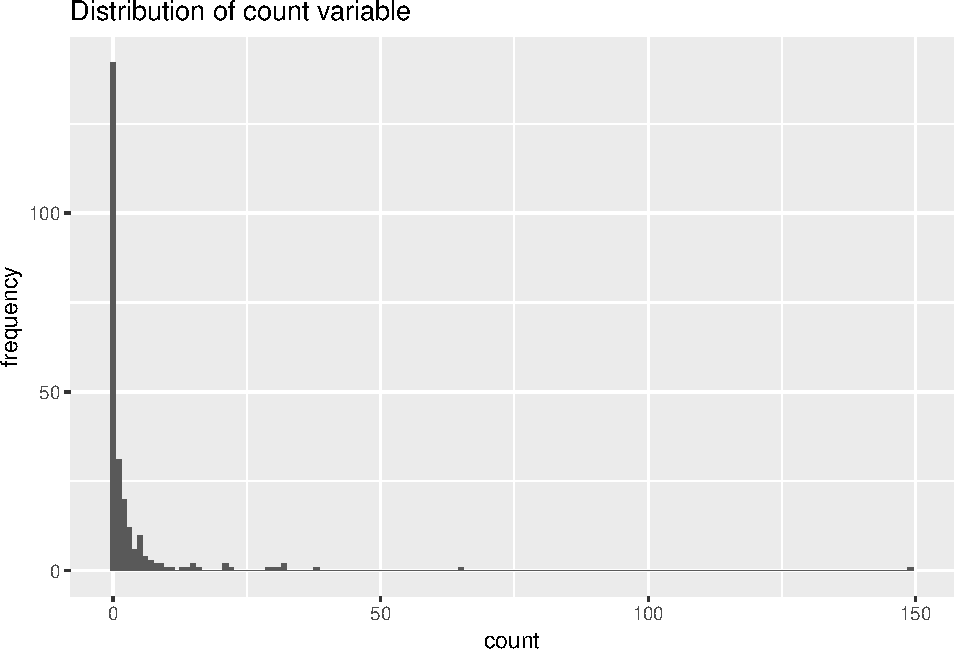
\includegraphics{05-poisreg_files/figure-latex/hist-1.pdf}

Предположим, что переменная имеет распределение Пуассона. Будем использовать пуассоновскую регрессию.
\[
P(y=k)=exp(-\lambda) \lambda^k / k!
\]
где \(\lambda=\exp(b_1 +b_2*x)\)

\begin{Shaded}
\begin{Highlighting}[]
\NormalTok{poisson =}\StringTok{ }\KeywordTok{glm}\NormalTok{(count }\OperatorTok{~}\StringTok{ }\NormalTok{child }\OperatorTok{+}\StringTok{ }\NormalTok{camper }\OperatorTok{+}\StringTok{  }\NormalTok{persons, }\DataTypeTok{family =} \StringTok{"poisson"}\NormalTok{, }\DataTypeTok{data =}\NormalTok{ df)}
\KeywordTok{summary}\NormalTok{(poisson)}
\end{Highlighting}
\end{Shaded}

\begin{verbatim}

Call:
glm(formula = count ~ child + camper + persons, family = "poisson", 
    data = df)

Deviance Residuals: 
    Min       1Q   Median       3Q      Max  
-6.8096  -1.4431  -0.9060  -0.0406  16.1417  

Coefficients:
            Estimate Std. Error z value Pr(>|z|)    
(Intercept) -1.98183    0.15226  -13.02   <2e-16 ***
child       -1.68996    0.08099  -20.87   <2e-16 ***
camper1      0.93094    0.08909   10.45   <2e-16 ***
persons      1.09126    0.03926   27.80   <2e-16 ***
---
Signif. codes:  0 '***' 0.001 '**' 0.01 '*' 0.05 '.' 0.1 ' ' 1

(Dispersion parameter for poisson family taken to be 1)

    Null deviance: 2958.4  on 249  degrees of freedom
Residual deviance: 1337.1  on 246  degrees of freedom
AIC: 1682.1

Number of Fisher Scoring iterations: 6
\end{verbatim}

Посчитаем средний предельный эффект для каждой переменной.

\begin{Shaded}
\begin{Highlighting}[]
\KeywordTok{colMeans}\NormalTok{(}\KeywordTok{marginal_effects}\NormalTok{(poisson))}
\end{Highlighting}
\end{Shaded}

\begin{verbatim}
Error in marginal_effects(poisson): could not find function "marginal_effects"
\end{verbatim}

Однако, заметим, что дисперсия и среднее значение объясняемой переменной не равны, как это предполагает распределение Пуассона.

\begin{Shaded}
\begin{Highlighting}[]
\NormalTok{df }\OperatorTok\StringTok{ }\KeywordTok{group_by}\NormalTok{(camper) }\OperatorTok\StringTok{ }\KeywordTok{summarize}\NormalTok{(}\DataTypeTok{var =} \KeywordTok{var}\NormalTok{(count), }\DataTypeTok{mean =} \KeywordTok{mean}\NormalTok{(count))}
\end{Highlighting}
\end{Shaded}

\begin{verbatim}
# A tibble: 2 x 3
  camper   var  mean
  <fct>  <dbl> <dbl>
1 0       21.1  1.52
2 1      212.   4.54
\end{verbatim}

Оценим регрессию, предполагая отрицательное биномиальное распределение остатков. В этом случае, дисперсия распределения зависит от некоторого параметра и не равна среднему.

\begin{Shaded}
\begin{Highlighting}[]
\NormalTok{nb1 =}\StringTok{ }\KeywordTok{glm.nb}\NormalTok{(count }\OperatorTok{~}\StringTok{ }\NormalTok{child }\OperatorTok{+}\StringTok{ }\NormalTok{camper }\OperatorTok{+}\StringTok{  }\NormalTok{persons, }\DataTypeTok{data =}\NormalTok{ df)}
\KeywordTok{summary}\NormalTok{(nb1)}
\end{Highlighting}
\end{Shaded}

\begin{verbatim}

Call:
glm.nb(formula = count ~ child + camper + persons, data = df, 
    init.theta = 0.4635287626, link = log)

Deviance Residuals: 
    Min       1Q   Median       3Q      Max  
-1.6673  -0.9599  -0.6590  -0.0319   4.9433  

Coefficients:
            Estimate Std. Error z value Pr(>|z|)    
(Intercept)  -1.6250     0.3304  -4.918 8.74e-07 ***
child        -1.7805     0.1850  -9.623  < 2e-16 ***
camper1       0.6211     0.2348   2.645  0.00816 ** 
persons       1.0608     0.1144   9.273  < 2e-16 ***
---
Signif. codes:  0 '***' 0.001 '**' 0.01 '*' 0.05 '.' 0.1 ' ' 1

(Dispersion parameter for Negative Binomial(0.4635) family taken to be 1)

    Null deviance: 394.25  on 249  degrees of freedom
Residual deviance: 210.65  on 246  degrees of freedom
AIC: 820.44

Number of Fisher Scoring iterations: 1

              Theta:  0.4635 
          Std. Err.:  0.0712 

 2 x log-likelihood:  -810.4440 
\end{verbatim}

Попробуем исключить из модели переменную \texttt{camper} и сравним качество двух моделей.

\begin{Shaded}
\begin{Highlighting}[]
\NormalTok{nb2 =}\StringTok{ }\KeywordTok{update}\NormalTok{(nb1, . }\OperatorTok{~}\StringTok{ }\NormalTok{. }\OperatorTok{-}\StringTok{ }\NormalTok{camper)}
\KeywordTok{waldtest}\NormalTok{(nb1, nb2)}
\end{Highlighting}
\end{Shaded}

\begin{verbatim}
Wald test

Model 1: count ~ child + camper + persons
Model 2: count ~ child + persons
  Res.Df Df      F   Pr(>F)   
1    246                      
2    247 -1 6.9979 0.008686 **
---
Signif. codes:  0 '***' 0.001 '**' 0.01 '*' 0.05 '.' 0.1 ' ' 1
\end{verbatim}

Можем посмотреть на результаты модели с ``раздутыми нулями'' (zero-inflated). Они предполагают большую частоту нулевых наблюдений.

\begin{Shaded}
\begin{Highlighting}[]
\NormalTok{zero_infl =}\StringTok{ }\KeywordTok{zeroinfl}\NormalTok{(count }\OperatorTok{~}\StringTok{ }\NormalTok{child }\OperatorTok{+}\StringTok{ }\NormalTok{camper }\OperatorTok{|}\StringTok{ }\NormalTok{persons, }\DataTypeTok{data =}\NormalTok{ df, }\DataTypeTok{dist =} \StringTok{'negbin'}\NormalTok{)}
\end{Highlighting}
\end{Shaded}

\begin{verbatim}
Error in zeroinfl(count ~ child + camper | persons, data = df, dist = "negbin"): could not find function "zeroinfl"
\end{verbatim}

\begin{Shaded}
\begin{Highlighting}[]
\KeywordTok{summary}\NormalTok{(zero_infl)}
\end{Highlighting}
\end{Shaded}

\begin{verbatim}
Error in summary(zero_infl): object 'zero_infl' not found
\end{verbatim}

\hypertarget{-----1}{%
\subsubsection{То же самое в стате}\label{-----1}}

Загружаем данные и смотрим описательные статистики.

\begin{verbatim}
use fish.dta
summarize
\end{verbatim}

\begin{verbatim}
    Variable |        Obs        Mean    Std. Dev.       Min        Max
-------------+---------------------------------------------------------
      camper |        250        .588    .4931824          0          1
       child |        250        .684    .8503153          0          3
       count |        250       3.296    11.63503          0        149
     persons |        250       2.528     1.11273          1          4
\end{verbatim}

\begin{verbatim}
hist count
\end{verbatim}

\begin{verbatim}
(bin=15, start=0, width=9.9333333)
\end{verbatim}

Строим Пуассоновскую регрессию.
В описательных статистиках:
\(AIC = -2log(L) + 2k\)
\(AIC = -2log(L) + klog(N)\)

\begin{verbatim}
glm count camper child persons, family(poisson)
\end{verbatim}

\begin{verbatim}
Iteration 0:   log likelihood = -965.92815  
Iteration 1:   log likelihood = -837.97093  
Iteration 2:   log likelihood = -837.07307  
Iteration 3:   log likelihood = -837.07248  
Iteration 4:   log likelihood = -837.07248  

Generalized linear models                         No. of obs      =        250
Optimization     : ML                             Residual df     =        246
                                                  Scale parameter =          1
Deviance         =  1337.079644                   (1/df) Deviance =   5.435283
Pearson          =  2910.627049                   (1/df) Pearson  =   11.83182

Variance function: V(u) = u                       [Poisson]
Link function    : g(u) = ln(u)                   [Log]

                                                  AIC             =    6.72858
Log likelihood   = -837.0724803                   BIC             =  -21.19974

------------------------------------------------------------------------------
             |                 OIM
       count |      Coef.   Std. Err.      z    P>|z|     [95% Conf. Interval]
-------------+----------------------------------------------------------------
      camper |   .9309359   .0890869    10.45   0.000     .7563289    1.105543
       child |  -1.689957   .0809922   -20.87   0.000    -1.848699   -1.531215
     persons |   1.091262   .0392553    27.80   0.000     1.014323    1.168201
       _cons |  -1.981827    .152263   -13.02   0.000    -2.280257   -1.683397
------------------------------------------------------------------------------
\end{verbatim}

Можем посчитать AIC и BIC по другой формуле, аналогично выводу R.
\(AIC = \frac {-2log(L) + 2k}{N}\)

\begin{verbatim}
estat ic
\end{verbatim}

\begin{verbatim}
Akaike's information criterion and Bayesian information criterion

-----------------------------------------------------------------------------
       Model |        Obs  ll(null)  ll(model)      df         AIC        BIC
-------------+---------------------------------------------------------------
           . |        250         .  -837.0725       4    1682.145   1696.231
-----------------------------------------------------------------------------
               Note: N=Obs used in calculating BIC; see [R] BIC note.
\end{verbatim}

Посмотрим, равны ли среднее значение и дисперсия, как это предполагает распределение Пуассона.

\begin{verbatim}
tabstat count, by(camper) stat(mean, variance) nototal
\end{verbatim}

\begin{verbatim}
Summary for variables: count
     by categories of: camper (CAMPER)

  camper |      mean  variance
---------+--------------------
       0 |  1.524272  21.05578
       1 |  4.537415   212.401
------------------------------
\end{verbatim}

Предположим, что остатки имеют отрицательное биномиальное распределение.

\begin{verbatim}
nbreg count child camper persons
\end{verbatim}

\begin{verbatim}
Fitting Poisson model:

Iteration 0:   log likelihood = -841.58831  
Iteration 1:   log likelihood = -837.07386  
Iteration 2:   log likelihood = -837.07248  
Iteration 3:   log likelihood = -837.07248  

Fitting constant-only model:

Iteration 0:   log likelihood = -582.76028  
Iteration 1:   log likelihood = -464.44518  
Iteration 2:   log likelihood = -464.43931  
Iteration 3:   log likelihood = -464.43931  

Fitting full model:

Iteration 0:   log likelihood = -438.02759  
Iteration 1:   log likelihood = -409.71171  
Iteration 2:   log likelihood = -405.34765  
Iteration 3:   log likelihood = -405.22204  
Iteration 4:   log likelihood =   -405.222  
Iteration 5:   log likelihood =   -405.222  

Negative binomial regression                    Number of obs     =        250
                                                LR chi2(3)        =     118.43
Dispersion     = mean                           Prob > chi2       =     0.0000
Log likelihood =   -405.222                     Pseudo R2         =     0.1275

------------------------------------------------------------------------------
       count |      Coef.   Std. Err.      z    P>|z|     [95% Conf. Interval]
-------------+----------------------------------------------------------------
       child |   -1.78052   .1920379    -9.27   0.000    -2.156907   -1.404132
      camper |   .6211286   .2358072     2.63   0.008      .158955    1.083302
     persons |     1.0608   .1174733     9.03   0.000     .8305564    1.291043
       _cons |   -1.62499   .3294006    -4.93   0.000    -2.270603   -.9793765
-------------+----------------------------------------------------------------
    /lnalpha |   .7688868   .1538497                      .4673469    1.070427
-------------+----------------------------------------------------------------
       alpha |   2.157363   .3319098                      1.595755    2.916624
------------------------------------------------------------------------------
LR test of alpha=0: chibar2(01) = 863.70               Prob >= chibar2 = 0.000
\end{verbatim}

Проверим гипотезу о равенстве 0 коэффицинта при переменной \texttt{camper}. Проведем тест Вальда.

\begin{verbatim}
quietly: nbreg count child i.camper persons #скрыть вывод регрессии
test i.camper 
\end{verbatim}

\begin{verbatim}
# invalid name
r(198);

end of do-file
r(198);
\end{verbatim}

Посчитаем средний предельный эффект для каждоый переменной.

\begin{verbatim}
margins, dydx(*)
\end{verbatim}

\begin{verbatim}
 # invalid name
r(198);



Average marginal effects                        Number of obs     =        250
Model VCE    : OIM

Expression   : Predicted number of events, predict()
dy/dx w.r.t. : child camper persons

------------------------------------------------------------------------------
             |            Delta-method
             |      dy/dx   Std. Err.      z    P>|z|     [95% Conf. Interval]
-------------+----------------------------------------------------------------
       child |  -5.842234   1.494053    -3.91   0.000    -8.770524   -2.913943
      camper |   2.038045   .8917015     2.29   0.022     .2903418    3.785748
     persons |   3.480692   .9200607     3.78   0.000     1.677406    5.283978
------------------------------------------------------------------------------
\end{verbatim}

И модель с раздутыми нулями.

\begin{verbatim}
zinb count child i.camper, inflate(persons)
\end{verbatim}

\begin{verbatim}
 # invalid name
r(198);



Fitting constant-only model:

Iteration 0:   log likelihood = -519.33992  
Iteration 1:   log likelihood = -471.96077  
Iteration 2:   log likelihood = -465.38193  
Iteration 3:   log likelihood = -464.39882  
Iteration 4:   log likelihood = -463.92704  
Iteration 5:   log likelihood = -463.79248  
Iteration 6:   log likelihood = -463.75773  
Iteration 7:   log likelihood =  -463.7518  
Iteration 8:   log likelihood = -463.75119  
Iteration 9:   log likelihood = -463.75118  

Fitting full model:

Iteration 0:   log likelihood = -463.75118  (not concave)
Iteration 1:   log likelihood = -440.43162  
Iteration 2:   log likelihood = -434.96651  
Iteration 3:   log likelihood = -433.49903  
Iteration 4:   log likelihood = -432.89949  
Iteration 5:   log likelihood = -432.89091  
Iteration 6:   log likelihood = -432.89091  

Zero-inflated negative binomial regression      Number of obs     =        250
                                                Nonzero obs       =        108
                                                Zero obs          =        142

Inflation model = logit                         LR chi2(2)        =      61.72
Log likelihood  = -432.8909                     Prob > chi2       =     0.0000

------------------------------------------------------------------------------
       count |      Coef.   Std. Err.      z    P>|z|     [95% Conf. Interval]
-------------+----------------------------------------------------------------
count        |
       child |  -1.515255   .1955912    -7.75   0.000    -1.898606   -1.131903
       _cons |   1.371048   .2561131     5.35   0.000     .8690758    1.873021
-------------+----------------------------------------------------------------
inflate      |
     persons |  -1.666563   .6792833    -2.45   0.014    -2.997934   -.3351922
       _cons |   1.603104   .8365065     1.92   0.055     -.036419    3.242626
-------------+----------------------------------------------------------------
    /lnalpha |   .9853533     .17595     5.60   0.000     .6404975    1.330209
-------------+----------------------------------------------------------------
       alpha |   2.678758   .4713275                      1.897425    3.781834
------------------------------------------------------------------------------
\end{verbatim}

\hypertarget{----python}{%
\subsubsection{То же самое в python}\label{----python}}

Нужные пакетики:

\begin{Shaded}
\begin{Highlighting}[]
\ImportTok{import}\NormalTok{ seaborn }\ImportTok{as}\NormalTok{ sns}
\ImportTok{import}\NormalTok{ matplotlib.pyplot }\ImportTok{as}\NormalTok{ plt}
\ImportTok{import}\NormalTok{ numpy }\ImportTok{as}\NormalTok{ np}
\ImportTok{import}\NormalTok{ pandas }\ImportTok{as}\NormalTok{ pd}
\NormalTok{plt.style.use(}\StringTok{'ggplot'}\NormalTok{)}
\end{Highlighting}
\end{Shaded}

Загружаем данные и смотрим описательные статистики.

\begin{Shaded}
\begin{Highlighting}[]
\NormalTok{df_fish }\OperatorTok{=}\NormalTok{ pd.read_stata(}\StringTok{'fish.dta'}\NormalTok{)}
\end{Highlighting}
\end{Shaded}

\begin{Shaded}
\begin{Highlighting}[]
\NormalTok{sns.distplot(df_fish[}\StringTok{'count'}\NormalTok{])}
\NormalTok{plt.show()}
\end{Highlighting}
\end{Shaded}

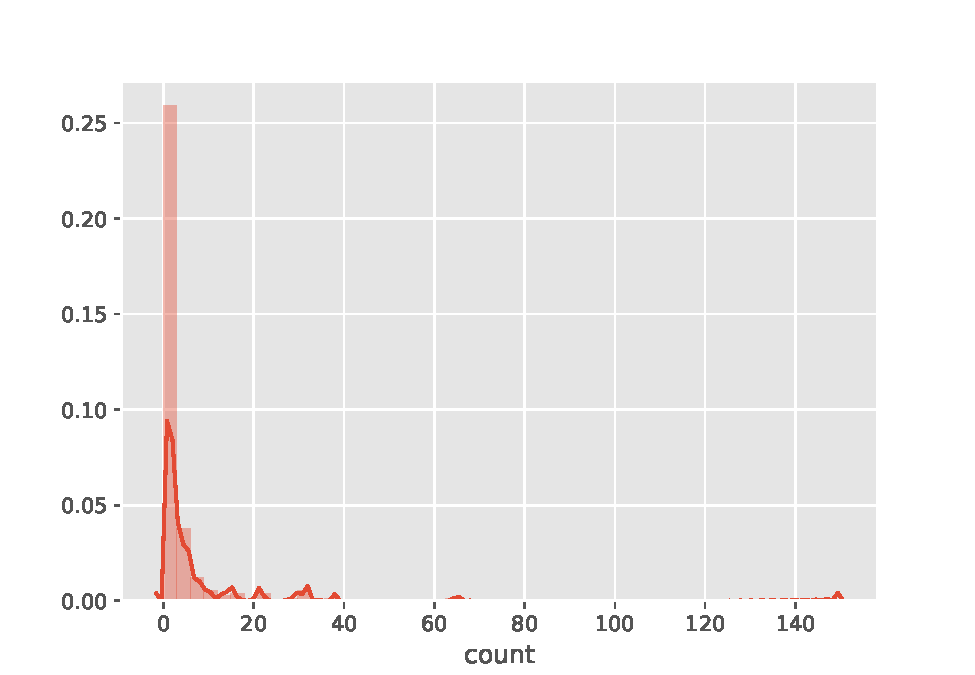
\includegraphics{05-poisreg_files/figure-latex/unnamed-chunk-12-1.pdf}

Превращаем переменную \texttt{camper} в категориальную.

\begin{Shaded}
\begin{Highlighting}[]
\NormalTok{df_fish[}\StringTok{'camper'}\NormalTok{]}\OperatorTok{=}\NormalTok{df_fish[}\StringTok{'camper'}\NormalTok{].astype(}\StringTok{'category'}\NormalTok{)}
\end{Highlighting}
\end{Shaded}

Строим Пуассоновскую регрессию.

\begin{Shaded}
\begin{Highlighting}[]
\NormalTok{regr_pois }\OperatorTok{=}\NormalTok{ smf.glm(}\StringTok{'count ~ child + camper +  persons'}\NormalTok{, data}\OperatorTok{=}\NormalTok{df_fish,}
\NormalTok{                    family}\OperatorTok{=}\NormalTok{sm.families.Poisson(link}\OperatorTok{=}\NormalTok{sm.families.links.log)).fit()}
\end{Highlighting}
\end{Shaded}

\begin{verbatim}
Error in py_call_impl(callable, dots$args, dots$keywords): NameError: name 'smf' is not defined

Detailed traceback: 
  File "<string>", line 1, in <module>
\end{verbatim}

\begin{Shaded}
\begin{Highlighting}[]
\NormalTok{regr_pois.summary()}
\end{Highlighting}
\end{Shaded}

\begin{verbatim}
Error in py_call_impl(callable, dots$args, dots$keywords): NameError: name 'regr_pois' is not defined

Detailed traceback: 
  File "<string>", line 1, in <module>
\end{verbatim}

Посмотрим, равны ли среднее значение и дисперсия, как это предполагает распределение Пуассона.

\begin{Shaded}
\begin{Highlighting}[]
\NormalTok{(df_fish}
\NormalTok{ .}\BuiltInTok{filter}\NormalTok{([}\StringTok{'count'}\NormalTok{, }\StringTok{'camper'}\NormalTok{])}
\NormalTok{ .groupby(}\StringTok{'camper'}\NormalTok{)}
\NormalTok{ .agg([}\StringTok{'mean'}\NormalTok{, }\StringTok{'var'}\NormalTok{]))}
\end{Highlighting}
\end{Shaded}

\begin{verbatim}
           count            
            mean         var
camper                      
0       1.524272   21.055778
1       4.537415  212.400988
\end{verbatim}

И регрессию с остатками, имеющими отрицательное биномиальное распределение.

\begin{Shaded}
\begin{Highlighting}[]
\NormalTok{regr_bin }\OperatorTok{=}\NormalTok{ smf.glm(}\StringTok{'count ~ child + camper +  persons'}\NormalTok{, data}\OperatorTok{=}\NormalTok{df_fish,}
\NormalTok{              family}\OperatorTok{=}\NormalTok{sm.families.NegativeBinomial(link}\OperatorTok{=}\NormalTok{sm.families.links.log)).fit()}
\end{Highlighting}
\end{Shaded}

\begin{verbatim}
Error in py_call_impl(callable, dots$args, dots$keywords): NameError: name 'smf' is not defined

Detailed traceback: 
  File "<string>", line 1, in <module>
\end{verbatim}

Проверим гипотезу о равенстве 0 коэффициента при переменной \texttt{camper}. Проведем тест Вальда.

\begin{Shaded}
\begin{Highlighting}[]
\NormalTok{hyp }\OperatorTok{=} \StringTok{'(camper = 0)'}
\NormalTok{regr_bin.wald_test(hyp)}
\end{Highlighting}
\end{Shaded}

\begin{verbatim}
Error in py_call_impl(callable, dots$args, dots$keywords): NameError: name 'regr_bin' is not defined

Detailed traceback: 
  File "<string>", line 1, in <module>
\end{verbatim}

Посчитаем средний предельный эффект для каждой переменной.

\begin{Shaded}
\begin{Highlighting}[]
\NormalTok{pred }\OperatorTok{=}\NormalTok{ regr_pois.fittedvalues}
\end{Highlighting}
\end{Shaded}

\begin{verbatim}
Error in py_call_impl(callable, dots$args, dots$keywords): NameError: name 'regr_pois' is not defined

Detailed traceback: 
  File "<string>", line 1, in <module>
\end{verbatim}

\begin{Shaded}
\begin{Highlighting}[]
\NormalTok{mean_mef_child }\OperatorTok{=}\NormalTok{ np.mean([regr_pois.params[}\DecValTok{1}\NormalTok{] }\OperatorTok{*}\NormalTok{ p }\ControlFlowTok{for}\NormalTok{ p }\KeywordTok{in}\NormalTok{ pred])}
\end{Highlighting}
\end{Shaded}

\begin{verbatim}
Error in py_call_impl(callable, dots$args, dots$keywords): NameError: name 'pred' is not defined

Detailed traceback: 
  File "<string>", line 1, in <module>
\end{verbatim}

\begin{Shaded}
\begin{Highlighting}[]
\NormalTok{mean_mef_camper }\OperatorTok{=}\NormalTok{ np.mean([regr_pois.params[}\DecValTok{2}\NormalTok{] }\OperatorTok{*}\NormalTok{ p }\ControlFlowTok{for}\NormalTok{ p }\KeywordTok{in}\NormalTok{ pred])}
\end{Highlighting}
\end{Shaded}

\begin{verbatim}
Error in py_call_impl(callable, dots$args, dots$keywords): NameError: name 'pred' is not defined

Detailed traceback: 
  File "<string>", line 1, in <module>
\end{verbatim}

\begin{Shaded}
\begin{Highlighting}[]
\NormalTok{data_1 }\OperatorTok{=}\NormalTok{ pd.DataFrame(\{}\StringTok{'child'}\NormalTok{: df_fish[}\StringTok{'child'}\NormalTok{], }\StringTok{'camper'}\NormalTok{: }\DecValTok{1}\NormalTok{, }\StringTok{'persons'}\NormalTok{: df_fish[}\StringTok{'persons'}\NormalTok{]\})}
\NormalTok{data_0 }\OperatorTok{=}\NormalTok{ pd.DataFrame(\{}\StringTok{'child'}\NormalTok{: df_fish[}\StringTok{'child'}\NormalTok{], }\StringTok{'camper'}\NormalTok{: }\DecValTok{0}\NormalTok{, }\StringTok{'persons'}\NormalTok{: df_fish[}\StringTok{'persons'}\NormalTok{]\})}
\NormalTok{mean_mef_persons }\OperatorTok{=}\NormalTok{ np.mean([(regr_pois.predict(data_1)[i]}\OperatorTok{-}\NormalTok{regr_pois.predict(data_0)[i]) }
                            \ControlFlowTok{for}\NormalTok{ i }\KeywordTok{in} \BuiltInTok{range}\NormalTok{(}\BuiltInTok{len}\NormalTok{(df_fish))])}
\end{Highlighting}
\end{Shaded}

\begin{verbatim}
Error in py_call_impl(callable, dots$args, dots$keywords): NameError: name 'regr_pois' is not defined

Detailed traceback: 
  File "<string>", line 2, in <module>
  File "<string>", line 2, in <listcomp>
\end{verbatim}

И модель с раздутыми нулями.

\begin{Shaded}
\begin{Highlighting}[]
\DecValTok{1}
\end{Highlighting}
\end{Shaded}

\begin{verbatim}
1
\end{verbatim}

Проблемы:

\begin{enumerate}
\def\labelenumi{\arabic{enumi})}
\setcounter{enumi}{1}
\tightlist
\item
  предельные эффекты в Питоне
\item
  clogit ВООБЩЕ НЕ ПОЛУЧАЕТСЯ
\end{enumerate}

\hypertarget{disordered}{%
\chapter{Модели неупорядоченного выбора}\label{disordered}}

\hypertarget{instruments}{%
\chapter{Интcтрументы для простой регрессии}\label{instruments}}

\hypertarget{arma}{%
\chapter{ARMA}\label{arma}}

\hypertarget{paneldata}{%
\chapter{Панельные данные}\label{paneldata}}

\hypertarget{heterosked}{%
\chapter{Гетероскедастичность в простой регрессии}\label{heterosked}}

\hypertarget{pca}{%
\chapter{PCA}\label{pca}}

\hypertarget{dinpanel}{%
\chapter{Динамические панели}\label{dinpanel}}

\hypertarget{tobit_heckit}{%
\chapter{TOBIT, HECKIT}\label{tobit_heckit}}

\hypertarget{treatment}{%
\chapter{Treatment effect}\label{treatment}}

\hypertarget{compatability}{%
\chapter{Что-то там про совместимость и языки}\label{compatability}}

\hypertarget{dict}{%
\chapter{Словарь}\label{dict}}

\bibliography{book.bib,packages.bib}


\end{document}
